\documentclass[]{article}
\usepackage{lmodern}
\usepackage{amssymb,amsmath}
\usepackage{ifxetex,ifluatex}
\usepackage{fixltx2e} % provides \textsubscript
\ifnum 0\ifxetex 1\fi\ifluatex 1\fi=0 % if pdftex
  \usepackage[T1]{fontenc}
  \usepackage[utf8]{inputenc}
\else % if luatex or xelatex
  \ifxetex
    \usepackage{mathspec}
    \usepackage{xltxtra,xunicode}
  \else
    \usepackage{fontspec}
  \fi
  \defaultfontfeatures{Mapping=tex-text,Scale=MatchLowercase}
  \newcommand{\euro}{€}
\fi
% use upquote if available, for straight quotes in verbatim environments
\IfFileExists{upquote.sty}{\usepackage{upquote}}{}
% use microtype if available
\IfFileExists{microtype.sty}{%
\usepackage{microtype}
\UseMicrotypeSet[protrusion]{basicmath} % disable protrusion for tt fonts
}{}
\usepackage[margin=1in]{geometry}
\usepackage{color}
\usepackage{fancyvrb}
\newcommand{\VerbBar}{|}
\newcommand{\VERB}{\Verb[commandchars=\\\{\}]}
\DefineVerbatimEnvironment{Highlighting}{Verbatim}{commandchars=\\\{\}}
% Add ',fontsize=\small' for more characters per line
\usepackage{framed}
\definecolor{shadecolor}{RGB}{248,248,248}
\newenvironment{Shaded}{\begin{snugshade}}{\end{snugshade}}
\newcommand{\KeywordTok}[1]{\textcolor[rgb]{0.13,0.29,0.53}{\textbf{{#1}}}}
\newcommand{\DataTypeTok}[1]{\textcolor[rgb]{0.13,0.29,0.53}{{#1}}}
\newcommand{\DecValTok}[1]{\textcolor[rgb]{0.00,0.00,0.81}{{#1}}}
\newcommand{\BaseNTok}[1]{\textcolor[rgb]{0.00,0.00,0.81}{{#1}}}
\newcommand{\FloatTok}[1]{\textcolor[rgb]{0.00,0.00,0.81}{{#1}}}
\newcommand{\CharTok}[1]{\textcolor[rgb]{0.31,0.60,0.02}{{#1}}}
\newcommand{\StringTok}[1]{\textcolor[rgb]{0.31,0.60,0.02}{{#1}}}
\newcommand{\CommentTok}[1]{\textcolor[rgb]{0.56,0.35,0.01}{\textit{{#1}}}}
\newcommand{\OtherTok}[1]{\textcolor[rgb]{0.56,0.35,0.01}{{#1}}}
\newcommand{\AlertTok}[1]{\textcolor[rgb]{0.94,0.16,0.16}{{#1}}}
\newcommand{\FunctionTok}[1]{\textcolor[rgb]{0.00,0.00,0.00}{{#1}}}
\newcommand{\RegionMarkerTok}[1]{{#1}}
\newcommand{\ErrorTok}[1]{\textbf{{#1}}}
\newcommand{\NormalTok}[1]{{#1}}
\usepackage{longtable,booktabs}
\usepackage{graphicx}
\makeatletter
\def\maxwidth{\ifdim\Gin@nat@width>\linewidth\linewidth\else\Gin@nat@width\fi}
\def\maxheight{\ifdim\Gin@nat@height>\textheight\textheight\else\Gin@nat@height\fi}
\makeatother
% Scale images if necessary, so that they will not overflow the page
% margins by default, and it is still possible to overwrite the defaults
% using explicit options in \includegraphics[width, height, ...]{}
\setkeys{Gin}{width=\maxwidth,height=\maxheight,keepaspectratio}
\ifxetex
  \usepackage[setpagesize=false, % page size defined by xetex
              unicode=false, % unicode breaks when used with xetex
              xetex]{hyperref}
\else
  \usepackage[unicode=true]{hyperref}
\fi
\hypersetup{breaklinks=true,
            bookmarks=true,
            pdfauthor={Derek G. Nokes, CUNY},
            pdftitle={Diversification in the Managed Futures Universe},
            colorlinks=true,
            citecolor=blue,
            urlcolor=blue,
            linkcolor=magenta,
            pdfborder={0 0 0}}
\urlstyle{same}  % don't use monospace font for urls
\setlength{\parindent}{0pt}
\setlength{\parskip}{6pt plus 2pt minus 1pt}
\setlength{\emergencystretch}{3em}  % prevent overfull lines
\setcounter{secnumdepth}{0}

%%% Use protect on footnotes to avoid problems with footnotes in titles
\let\rmarkdownfootnote\footnote%
\def\footnote{\protect\rmarkdownfootnote}

%%% Change title format to be more compact
\usepackage{titling}
\setlength{\droptitle}{-2em}
  \title{Diversification in the Managed Futures Universe}
  \pretitle{\vspace{\droptitle}\centering\huge}
  \posttitle{\par}
  \author{Derek G. Nokes, CUNY}
  \preauthor{\centering\large\emph}
  \postauthor{\par}
  \predate{\centering\large\emph}
  \postdate{\par}
  \date{Friday, May 22, 2015}




\begin{document}

\maketitle


{
\hypersetup{linkcolor=black}
\setcounter{tocdepth}{3}
\tableofcontents
}
```

\pagebreak

\section{Abstract}\label{abstract}

In this paper, we focus on the application of a statistical factor model
to a subset of the universe of managed futures investment programs. Our
objective is to model the relationships between the returns of a select
set of these investment programs and to produce a simple sensitivity
providing a map of the return variability of a portfolio to changes in
the diversity of the portfolio components as represented by the
\emph{importance} of a few factors. The paper is composed of four main
sections encompassing the entire data science workflow.

-- Section 1: Introduction and Motivation

-- Section 2: Data

\begin{itemize}
\item
  Raw Data Extraction, Transformation, and Loading (ETL)
\item
  Data Exploration
\item
  Data Cleaning
\end{itemize}

-- Section 3: Modeling

\begin{itemize}
\item
  Theory
\item
  Application
\end{itemize}

-- Section 4: Conclusions

\pagebreak

\section{Introduction and Motivation}\label{introduction-and-motivation}

In portfolio allocation applications the objective is to maximize
investors' future wealth by determining how to allocate capital among a
set of available investments in such a way as to maximize
\emph{compound} growth subject to a set of constraints. Maximizing
wealth requires that we take advantage of the powerful positive effects
of compounding. When we reinvest, the magnitude of investment returns
and the variability of those returns make \emph{equal} contributions to
compounded total return. Reducing the variability of returns thus has as
much impact on total return as the magnitude of returns. The variability
of portfolio return is a function of the co-variability of investment
component returns. If the component returns tend to move together, the
magnitude of fluctuations in the monthly value of the portfolio is
higher than if the components move in different directions. A portfolio
comprised of components with diversified returns will achieve higher
compound growth than a portfolio with less diversified components
holding average component returns constant. In the simplest terms,
portfolio allocation is primarily about selecting sets of investments
with \emph{future} positive average returns and low co-variability.

As the size of a portfolio increases, the number of inter-relationships
between components explodes. It becomes increasingly difficult to
understand the drivers of portfolio return as the number of components
rises because the number of independent parameters in a covariance
matrix grows with the square of the number of investments. Grouping
investments that tend to move together and focusing on trying to find
groups that are independent is one common way to reduce the dimension of
the portfolio allocation problem. This can be accomplished through the
use of statistical \emph{factor models}.

\subsection{Portfolio Return \& Its
Variability}\label{portfolio-return-its-variability}

In this section, we introduce definitions for portfolio return and
variability that will be used throughout the paper.

\subsubsection{Portfolio Return}\label{portfolio-return}

Portfolio return is a function of the weights and the returns of
portfolio investment components. We define the portfolio return for
\(I\) component investments for the month \(m\) given the monthly
returns and portfolio weights for each component investment \(i\) as:

\[r_{P,m}=\sum_{i=1}^{I}\left(r_{i,m}w_{i,m}\right)\]

Letting \(W_{m}\) be a vector of portfolio component weights for month
\(m\), \(T\) denote the transpose operator, and \(R_{m}\) be a vector of
the month \(m\) component returns, we can use matrix notation to define
the portfolio return as follows:

\[r_{P,m}=W^{T}R\]

The holdig period return (HPR) for the portfolio is one plus the
portfolio return for the month \(m\):

\[HPR_{P,m}=1+\sum_{i=1}^{I}\left(r_{i,m}w_{i,m}\right)=1+r_{P,m}\]

The holding period return is the factor by which we mulitply the
starting value of the portfolio to get the ending value of a portfolio,
given the monthly returns and weights of each component investment.

Similarly, we define the terminal wealth relative (TWR) as the factor by
which we multiply the starting value of the portfolio to get the ending
value of the portfolio given the return streams and weights for a
sequence of months between one and \(M\):

\[TWR_{P,M}=\prod_{1=m}^{M}\left(1+\left(\sum_{i=1}^{I}\left(r_{i,m}w_{i,m}\right)\right)\right)=\prod_{1=m}^{M}HPR_{P,m}\]

We define the portfolio compounded return for the interval from months
one and \(M\) as the portfolio terminal wealth relative minus one:

\[r_{P,M}=\left(\prod_{1=m}^{M}\left(1+\left(\sum_{i=1}^{I}\left(r_{i,m}w_{i,m}\right)\right)\right)\right)-1=\left(\prod_{1=m}^{M}\left(1+r_{P,m}\right)\right)-1=\left(\prod_{1=m}^{M}HPR_{P,m}\right)-1=TWR_{P,M}-1\]

\subsubsection{Portfolio Return
Variability}\label{portfolio-return-variability}

Assuming that component returns are normally distributed, and thus that
components returns are multivariate normally distributed, we can define
the standard deviation of the portfolio returns using matrix notation
as:

\[\sigma_{P,M}=\sqrt{Var\left( {W_{m}}^{T} R_{m} \right)}=\sqrt{{W_{m}}^T\Sigma W_{m}}\]

Where \(W_{m}\) is a vector of portfolio component weights for month
\(m\), \(T\) denotes the transpose operator, \(R_{m}\) is a vector of
the month \(m\) component returns, and \(\Sigma\) is the return
covariance matrix.

\begin{Shaded}
\begin{Highlighting}[]
\NormalTok{portfolioVolatility <-}\StringTok{ }\NormalTok{function (W,COV)\{}
  \NormalTok{portfolioStandardDeviation =}\StringTok{ }\KeywordTok{sqrt}\NormalTok{( }\KeywordTok{t}\NormalTok{(W)%*%COV%*%W )  }
\NormalTok{\}}
\end{Highlighting}
\end{Shaded}

\subsubsection{Portfolio Return Confidence
Intervals:}\label{portfolio-return-confidence-intervals}

Using our definition of portfolio return variability we can define the
expected negative fluctuation (i.e., loss) at a given confidence
interval as:

\[VaR = -\alpha_{CL}\sigma_{P,M}\]

Where

\(\alpha_{CL}\) is the critical value at the confidence level \(CL\)

\(\sigma_{P,M}\) is the standard deviation of the portfolio returns over
the time interval \(m=1, \dots, M\)

This simple parameteric model can be extended in a myriad of ways to
account for the established stylized facts pertaining to the statistical
characteristics of investment returns. In particular, our factor-based
model can be combined with any choice for the the marginal distribution
of component returns, copulas can be used to include more extreme
returns in the joint distribution of returns, and returns can be
standardized wtih forecasts of the time-varying moments about the
distribution. In this paper, we focus on the simplest possible model for
the expected return distribution so that we may focus specifically on
the factor model.

\subsection{Too Many Moving Parts}\label{too-many-moving-parts}

The number of independent parameters \(P\) in a covariance matrix grows
with the number of investments \(I\) according to the following
function:

\[P=\frac{I\left(I+1\right)}{2}\]

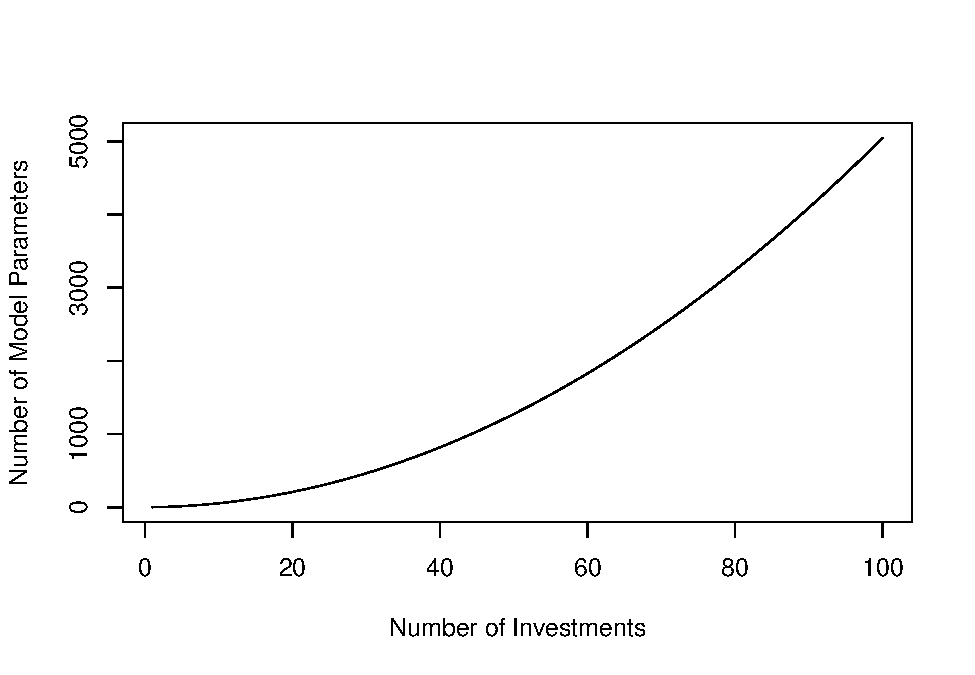
\includegraphics{diversificationInTheManagedFuturesUniverse_files/figure-latex/unnamed-chunk-6-1.pdf}

The number of independent parameters to be estimated in the covariance
matrix grows with the square of the number of investments, while the
number of data points available to estimate a covariance matrix grows
only linearly with the number of investments. In other words, the larger
the portfolio, the more historical data we typically need to estimate
the covariance matrix reliably. This is particularly problematic when
our interest is in the temporal evolution of the relationships between
investments in the portfolio.

In this paper, we extract the manager, program, and monthly return data
for the subset of the managed futures investment universe tracked on the
Altergris website. We conduct some limited exploratory data analysis and
clean the data to be used in our modeling. We create a statistical
factor model using principal component analysis (PCA), then use our
statistical factor model to group and interpret the relationships
between available programs in the managed futures investment universe.
Finally, we compute sensitivities linking the portfolio volatility of a
hypothetical set of managed futures investments to changes in the
importance of different factors. The sensitivities provide a powerful
analytical framework to be used to understand portfolio return variation
in terms of a few independent factors.

\section{Data}\label{data}

In this section we provide detailed information about the acquisition of
the data for this paper. A brief overview of the available data is
provided below. It is important to note that much of the data collected
was ultimately not cleaned and used in modeling. Data in the database
has not been normalized as this application is not transaction oriented
and storage has been set-up for a one-time analysis.

Although return data quality appears high, the quality of data
pertaining to manager and program information is much lower. This data
set will likely be cleaned and used for future research projects. The
entire system for collecting and storing the data is included below.

\subsection{Raw Data Extraction, Transformation, and Loading
(ETL)}\label{raw-data-extraction-transformation-and-loading-etl}

We exract the raw manager, program, and monthly return data to
pipe-delimited flat files using some custom R functions made
considerably simpler through the use of the `rvest' and `lubridate'
packages.

for each managed futures program on the Altergis website we extract the
following types of information:

-- CTA Name

\begin{Shaded}
\begin{Highlighting}[]
\NormalTok{extractCtaName<-function (programHtmlSession)\{  }
  \CommentTok{# extract the CTA name}
  \NormalTok{ctaName <-}\StringTok{ }\NormalTok{programHtmlSession %>%}\StringTok{ }\KeywordTok{html}\NormalTok{() %>%}\StringTok{ }
\StringTok{    }\KeywordTok{html_nodes}\NormalTok{(}\StringTok{"#spnHeadingPP1"}\NormalTok{) %>%}\StringTok{ }\KeywordTok{html_text}\NormalTok{()}
  \CommentTok{# remove foreign language characters}
  \NormalTok{ctaName}
\NormalTok{\}}
\end{Highlighting}
\end{Shaded}

-- Program Name

\begin{Shaded}
\begin{Highlighting}[]
\NormalTok{extractProgramName<-function (programHtmlSession)\{  }
  \CommentTok{# extract the program name}
  \NormalTok{programName <-}\StringTok{ }\NormalTok{programHtmlSession %>%}\StringTok{ }\KeywordTok{html}\NormalTok{() %>%}\StringTok{ }
\StringTok{    }\KeywordTok{html_nodes}\NormalTok{(}\StringTok{"#spnHeadingPP2"}\NormalTok{) %>%}\StringTok{ }\KeywordTok{html_text}\NormalTok{()  }
  \CommentTok{# remove foreign language characters  }
  \NormalTok{programName}
\NormalTok{\}}
\end{Highlighting}
\end{Shaded}

-- Monthly Returns

\begin{Shaded}
\begin{Highlighting}[]
\NormalTok{extractMonthlyReturns<-function (programHtmlSession,programId)\{  }
  \CommentTok{# extract CTA Name}
  \NormalTok{ctaName<-}\KeywordTok{extractCtaName}\NormalTok{(programHtmlSession)}
  \CommentTok{# extract the program name}
  \NormalTok{programName<-}\KeywordTok{extractProgramName}\NormalTok{(programHtmlSession)}
  \CommentTok{# extract the monthly returns}
  \NormalTok{a<-}\KeywordTok{html_table}\NormalTok{(}\KeywordTok{html_nodes}\NormalTok{(programHtmlSession, }\StringTok{"table"}\NormalTok{)[[}\DecValTok{1}\NormalTok{]],}\DataTypeTok{fill=}\OtherTok{TRUE}\NormalTok{)}
  \CommentTok{# extract the years}
  \NormalTok{YYYY<-}\KeywordTok{as.numeric}\NormalTok{(a$X1[}\DecValTok{3}\NormalTok{:(}\KeywordTok{length}\NormalTok{(a$X1)-}\DecValTok{1}\NormalTok{)])}
  \CommentTok{# find the number of years}
  \NormalTok{nYears<-}\KeywordTok{length}\NormalTok{(YYYY)}
  \CommentTok{# create the empty end of month date matrix}
  \NormalTok{dates<-}\KeywordTok{matrix}\NormalTok{(}\DataTypeTok{data=}\OtherTok{NA}\NormalTok{,}\DataTypeTok{nrow=}\NormalTok{nYears,}\DataTypeTok{ncol=}\DecValTok{12}\NormalTok{)}
  \CommentTok{# find the last day of each month}
  \NormalTok{for (yyyyIndex in }\KeywordTok{seq_along}\NormalTok{(YYYY))\{ }
    \NormalTok{yyyy<-YYYY[yyyyIndex]}
    \CommentTok{# find the last day for the current year}
    \NormalTok{eomDates<-}\KeywordTok{ceiling_date}\NormalTok{(}\KeywordTok{ISOdate}\NormalTok{(yyyy,}\DecValTok{1}\NormalTok{,}\DecValTok{1}\NormalTok{,}\DecValTok{0}\NormalTok{,}\DecValTok{0}\NormalTok{,}\DecValTok{0}\NormalTok{,}\DataTypeTok{tz=}\StringTok{'EST'}\NormalTok{) +}\StringTok{ }
\StringTok{                             }\KeywordTok{months}\NormalTok{(}\DecValTok{1}\NormalTok{:}\DecValTok{12}\NormalTok{))-}\KeywordTok{days}\NormalTok{(}\DecValTok{1}\NormalTok{)}
    \CommentTok{# store the end of month dates}
    \NormalTok{dates[yyyyIndex,}\DecValTok{1}\NormalTok{:}\DecValTok{12}\NormalTok{]<-}\KeywordTok{format}\NormalTok{(eomDates, }\StringTok{'%Y-%m-%d'}\NormalTok{)}
  \NormalTok{\}}
  \CommentTok{# flatten the end of month matrix}
  \NormalTok{eomDates<-}\KeywordTok{matrix}\NormalTok{(dates,}\DataTypeTok{nrow=}\NormalTok{nYears*}\DecValTok{12}\NormalTok{,}\DecValTok{1}\NormalTok{)  }
  \CommentTok{# extract the returns}
  \NormalTok{jan<-}\KeywordTok{as.numeric}\NormalTok{(a$X2[!}\KeywordTok{is.na}\NormalTok{(}\KeywordTok{sub}\NormalTok{(}\StringTok{'Jan'}\NormalTok{,}\OtherTok{NA}\NormalTok{,a$X2))])}
  \NormalTok{feb<-}\KeywordTok{as.numeric}\NormalTok{(a$X3[!}\KeywordTok{is.na}\NormalTok{(}\KeywordTok{sub}\NormalTok{(}\StringTok{'Feb'}\NormalTok{,}\OtherTok{NA}\NormalTok{,a$X3))])}
  \NormalTok{mar<-}\KeywordTok{as.numeric}\NormalTok{(a$X4[!}\KeywordTok{is.na}\NormalTok{(}\KeywordTok{sub}\NormalTok{(}\StringTok{'Mar'}\NormalTok{,}\OtherTok{NA}\NormalTok{,a$X4))])}
  \NormalTok{apr<-}\KeywordTok{as.numeric}\NormalTok{(a$X5[!}\KeywordTok{is.na}\NormalTok{(}\KeywordTok{sub}\NormalTok{(}\StringTok{'Apr'}\NormalTok{,}\OtherTok{NA}\NormalTok{,a$X5))])}
  \NormalTok{may<-}\KeywordTok{as.numeric}\NormalTok{(a$X6[!}\KeywordTok{is.na}\NormalTok{(}\KeywordTok{sub}\NormalTok{(}\StringTok{'May'}\NormalTok{,}\OtherTok{NA}\NormalTok{,a$X6))])}
  \NormalTok{jun<-}\KeywordTok{as.numeric}\NormalTok{(a$X7[!}\KeywordTok{is.na}\NormalTok{(}\KeywordTok{sub}\NormalTok{(}\StringTok{'Jun'}\NormalTok{,}\OtherTok{NA}\NormalTok{,a$X7))])}
  \NormalTok{jul<-}\KeywordTok{as.numeric}\NormalTok{(a$X8[!}\KeywordTok{is.na}\NormalTok{(}\KeywordTok{sub}\NormalTok{(}\StringTok{'Jul'}\NormalTok{,}\OtherTok{NA}\NormalTok{,a$X8))])}
  \NormalTok{aug<-}\KeywordTok{as.numeric}\NormalTok{(a$X9[!}\KeywordTok{is.na}\NormalTok{(}\KeywordTok{sub}\NormalTok{(}\StringTok{'Aug'}\NormalTok{,}\OtherTok{NA}\NormalTok{,a$X9))])}
  \NormalTok{sep<-}\KeywordTok{as.numeric}\NormalTok{(a$X10[!}\KeywordTok{is.na}\NormalTok{(}\KeywordTok{sub}\NormalTok{(}\StringTok{'Sep'}\NormalTok{,}\OtherTok{NA}\NormalTok{,a$X10))])}
  \NormalTok{oct<-}\KeywordTok{as.numeric}\NormalTok{(a$X11[!}\KeywordTok{is.na}\NormalTok{(}\KeywordTok{sub}\NormalTok{(}\StringTok{'Oct'}\NormalTok{,}\OtherTok{NA}\NormalTok{,a$X11))])}
  \NormalTok{nov<-}\KeywordTok{as.numeric}\NormalTok{(a$X12[!}\KeywordTok{is.na}\NormalTok{(}\KeywordTok{sub}\NormalTok{(}\StringTok{'Nov'}\NormalTok{,}\OtherTok{NA}\NormalTok{,a$X12))])}
  \NormalTok{dec<-}\KeywordTok{as.numeric}\NormalTok{(a$X13[!}\KeywordTok{is.na}\NormalTok{(}\KeywordTok{sub}\NormalTok{(}\StringTok{'Dec'}\NormalTok{,}\OtherTok{NA}\NormalTok{,a$X13))])}
  \CommentTok{# create the monthly return data frame}
  \NormalTok{monthlyReturns<-}\KeywordTok{cbind}\NormalTok{(ctaName,programName,yyyy,jan,feb,mar,}
    \NormalTok{apr,may,jun,jul,aug,sep,oct,nov,dec)}
  \CommentTok{# create the monthly return matrix by year}
  \NormalTok{monthlyReturnsMatrix<-}\KeywordTok{as.matrix}\NormalTok{(}\KeywordTok{cbind}\NormalTok{(jan,feb,mar,apr,}
    \NormalTok{may,jun,jul,aug,sep,oct,nov,dec))}
  \CommentTok{# find the dimension of the monthly returns matrix}
  \NormalTok{dimension<-}\KeywordTok{dim}\NormalTok{(monthlyReturnsMatrix)}
  \CommentTok{# flatten the monthly return matrix}
  \NormalTok{monthlyReturnsData<-}\KeywordTok{matrix}\NormalTok{(monthlyReturnsMatrix,dimension[}\DecValTok{1}\NormalTok{]*dimension[}\DecValTok{2}\NormalTok{],}\DecValTok{1}\NormalTok{)}
  \CommentTok{# create the data frame}
  \NormalTok{data<-}\KeywordTok{data.frame}\NormalTok{(}\DataTypeTok{dates=}\NormalTok{eomDates,}\DataTypeTok{monthlyReturns=}\NormalTok{monthlyReturnsData,}
    \DataTypeTok{stringsAsFactors=}\OtherTok{FALSE}\NormalTok{)}
  \CommentTok{# get the sort index}
  \NormalTok{sortIndex<-}\KeywordTok{sort}\NormalTok{(data[,}\DecValTok{1}\NormalTok{],}\DataTypeTok{index.return=}\OtherTok{TRUE}\NormalTok{)}
  \CommentTok{# order the data}
  \NormalTok{data<-data[sortIndex$ix,]}
  \CommentTok{# add the CTA Name}
  \NormalTok{data[}\StringTok{'ctaName'}\NormalTok{]<-ctaName}
  \CommentTok{# add the program name}
  \NormalTok{data[}\StringTok{'programName'}\NormalTok{]<-programName}
  \CommentTok{# add the program ID}
  \NormalTok{data[}\StringTok{'programId'}\NormalTok{]<-programId}
  \CommentTok{# find the NAs}
  \NormalTok{naIndex<-}\KeywordTok{is.na}\NormalTok{(data[,}\DecValTok{2}\NormalTok{])}
  \CommentTok{# return the data}
  \NormalTok{data[!naIndex,]}
\NormalTok{\}}
\end{Highlighting}
\end{Shaded}

-- Manager Address

\begin{Shaded}
\begin{Highlighting}[]
\NormalTok{extractAddress<-function (programHtmlSession,ctaName,programName)\{  }
  \CommentTok{# extract the address}
  \NormalTok{address<-}\KeywordTok{html_table}\NormalTok{(}\KeywordTok{html_nodes}\NormalTok{(programHtmlSession, }
    \StringTok{"table"}\NormalTok{)[[}\DecValTok{10}\NormalTok{]],}\DataTypeTok{fill=}\OtherTok{TRUE}\NormalTok{)  }
  \CommentTok{# extract the address}
  \NormalTok{addressHeader<-}\KeywordTok{t}\NormalTok{(address[}\DecValTok{1}\NormalTok{])}
  \CommentTok{# remove the colons}
  \NormalTok{addressHeader<-}\KeywordTok{sub}\NormalTok{(}\StringTok{':'}\NormalTok{,}\StringTok{''}\NormalTok{,addressHeader[}\DecValTok{2}\NormalTok{:}\DecValTok{7}\NormalTok{])}
  \NormalTok{addressData<-}\KeywordTok{t}\NormalTok{(address[}\DecValTok{2}\NormalTok{])}
  \CommentTok{# remove new line characters}
  \NormalTok{addressData<-}\KeywordTok{sub}\NormalTok{(}\StringTok{'}\CharTok{\textbackslash{}n}\StringTok{'}\NormalTok{,}\StringTok{'-'}\NormalTok{,addressData[}\DecValTok{2}\NormalTok{:}\DecValTok{7}\NormalTok{])}
  \CommentTok{# create address data frame}
  \NormalTok{address<-}\KeywordTok{data.frame}\NormalTok{(}\KeywordTok{cbind}\NormalTok{(addressHeader,addressData))}
  \KeywordTok{colnames}\NormalTok{(address)<-}\KeywordTok{c}\NormalTok{(}\StringTok{'column'}\NormalTok{,}\StringTok{'value'}\NormalTok{)}
  \NormalTok{address[}\StringTok{'columnType'}\NormalTok{]<-}\StringTok{'address'}
  \NormalTok{address}
\NormalTok{\}}
\end{Highlighting}
\end{Shaded}

-- Investment Methodology

\begin{Shaded}
\begin{Highlighting}[]
\NormalTok{extractInvestmentMethodology<-function (programHtmlSession,ctaName,programName)\{ }
  \CommentTok{# extract the investment methodlogy}
  \NormalTok{investmentMethodology<-}\KeywordTok{html_table}\NormalTok{(}\KeywordTok{html_nodes}\NormalTok{(programHtmlSession,}
    \StringTok{"table"}\NormalTok{)[[}\DecValTok{14}\NormalTok{]])}
  \NormalTok{investmentMethodologyHeader<-}\KeywordTok{t}\NormalTok{(investmentMethodology[}\DecValTok{1}\NormalTok{])}
  \NormalTok{investmentMethodologyData<-}\KeywordTok{t}\NormalTok{(investmentMethodology[}\DecValTok{2}\NormalTok{])}
  \KeywordTok{colnames}\NormalTok{(investmentMethodology)<-}\KeywordTok{c}\NormalTok{(}\StringTok{'column'}\NormalTok{,}\StringTok{'value'}\NormalTok{)}
  \NormalTok{investmentMethodology[}\StringTok{'columnType'}\NormalTok{]<-}\StringTok{'investmentMethodology'}
  \NormalTok{investmentMethodology}
\NormalTok{\}}
\end{Highlighting}
\end{Shaded}

-- Instruments Traded

\begin{Shaded}
\begin{Highlighting}[]
\NormalTok{extractInstruments<-function (programHtmlSession,ctaName,programName)\{}
  \CommentTok{# extract the instruments}
  \NormalTok{instruments<-}\KeywordTok{html_table}\NormalTok{(}\KeywordTok{html_nodes}\NormalTok{(programHtmlSession, }
    \StringTok{"table"}\NormalTok{)[[}\DecValTok{15}\NormalTok{]])  }
  \KeywordTok{colnames}\NormalTok{(instruments)<-}\KeywordTok{c}\NormalTok{(}\StringTok{'column'}\NormalTok{,}\StringTok{'value'}\NormalTok{)}
  \NormalTok{instruments[}\StringTok{'columnType'}\NormalTok{]<-}\StringTok{'instruments'}
  \NormalTok{instruments}
\NormalTok{\}}
\end{Highlighting}
\end{Shaded}

-- Sectors of Instruments Traded

\begin{Shaded}
\begin{Highlighting}[]
\CommentTok{# extract program data}
\NormalTok{extractSectors<-function (programHtmlSession,ctaName,programName)\{  }
  \CommentTok{# extract sector information}
  \NormalTok{sectors<-}\KeywordTok{html_table}\NormalTok{(}\KeywordTok{html_nodes}\NormalTok{(programHtmlSession,}
    \StringTok{"table"}\NormalTok{)[[}\DecValTok{13}\NormalTok{]])  }
  \CommentTok{# extract sector information}
  \KeywordTok{colnames}\NormalTok{(sectors)<-}\KeywordTok{c}\NormalTok{(}\StringTok{'column'}\NormalTok{,}\StringTok{'value'}\NormalTok{)}
  \NormalTok{sectors[}\StringTok{'columnType'}\NormalTok{]<-}\StringTok{'sectors'}
  \NormalTok{sectors}
\NormalTok{\}}
\end{Highlighting}
\end{Shaded}

-- Geographical Focus of Instruments Traded

\begin{Shaded}
\begin{Highlighting}[]
\NormalTok{extractGeographicalFocus<-function (programHtmlSession)\{}
  \CommentTok{# extract the geographical focus}
  \NormalTok{geographicalFocus<-}\KeywordTok{html_table}\NormalTok{(}\KeywordTok{html_nodes}\NormalTok{(programHtmlSession, }
    \StringTok{"table"}\NormalTok{)[[}\DecValTok{16}\NormalTok{]])}
  \CommentTok{# extract the geographical focus}
  \KeywordTok{colnames}\NormalTok{(geographicalFocus)<-}\KeywordTok{c}\NormalTok{(}\StringTok{'column'}\NormalTok{,}\StringTok{'value'}\NormalTok{)}
  \NormalTok{geographicalFocus[}\StringTok{'columnType'}\NormalTok{]<-}\StringTok{'geographicalFocus'}
  \NormalTok{geographicalFocus}
\NormalTok{\}}
\end{Highlighting}
\end{Shaded}

-- Holding Periods (Short/Medium/Long)

\begin{Shaded}
\begin{Highlighting}[]
\NormalTok{extractHoldingPeriod<-function (programHtmlSession)\{  }
  \CommentTok{# extract the holding period}
  \NormalTok{holdingPeriod<-}\KeywordTok{html_table}\NormalTok{(}\KeywordTok{html_nodes}\NormalTok{(programHtmlSession,}
    \StringTok{"table"}\NormalTok{)[[}\DecValTok{17}\NormalTok{]])}
  \KeywordTok{colnames}\NormalTok{(holdingPeriod)<-}\KeywordTok{c}\NormalTok{(}\StringTok{'column'}\NormalTok{,}\StringTok{'value'}\NormalTok{)}
  \NormalTok{holdingPeriod[}\StringTok{'columnType'}\NormalTok{]<-}\StringTok{'holdingPeriod'}
  \NormalTok{holdingPeriod}
\NormalTok{\}}
\end{Highlighting}
\end{Shaded}

-- Investment Terms and Information

\begin{Shaded}
\begin{Highlighting}[]
\NormalTok{extractInvestmentTermsAndInfo<-function (programHtmlSession)\{  }
  \CommentTok{# extract the investment terms and info}
  \NormalTok{investmentTermsAndInfo<-}\KeywordTok{html_table}\NormalTok{(}\KeywordTok{html_nodes}\NormalTok{(programHtmlSession, }
    \StringTok{"table"}\NormalTok{)[[}\DecValTok{18}\NormalTok{]])}
  \NormalTok{investmentTermsAndInfo[,}\DecValTok{2}\NormalTok{]<-}\OtherTok{NULL}
  \KeywordTok{colnames}\NormalTok{(investmentTermsAndInfo)<-}\KeywordTok{c}\NormalTok{(}\StringTok{'column'}\NormalTok{,}\StringTok{'value'}\NormalTok{)}
  \NormalTok{investmentTermsAndInfo[}\StringTok{'columnType'}\NormalTok{]<-}\StringTok{'investmentTermsAndInfo'}
  \NormalTok{investmentTermsAndInfo}
\NormalTok{\}}
\end{Highlighting}
\end{Shaded}

We extract manager, program, and month return data for a single CTA
program with a function that calls functions for each sub-type.

\begin{Shaded}
\begin{Highlighting}[]
\CommentTok{# extract program data}
\NormalTok{extractProgramInfo<-function (programHtmlSession,programId)\{  }
  \CommentTok{# create the program session}
  \CommentTok{# extract the CTA name  }
  \NormalTok{ctaName<-}\KeywordTok{extractCtaName}\NormalTok{(programHtmlSession)}
  \CommentTok{# extract the program name}
  \NormalTok{programName<-}\KeywordTok{extractProgramName}\NormalTok{(programHtmlSession)}
  \CommentTok{# extract the address data into a data frame}
  \NormalTok{address<-}\KeywordTok{extractAddress}\NormalTok{(programHtmlSession)}
  \CommentTok{# extract the investment methodology data into a data frame}
  \NormalTok{investmentMethodology<-}\KeywordTok{extractInvestmentMethodology}\NormalTok{(programHtmlSession)}
  \CommentTok{# extract the instruments data into a data frame  }
  \NormalTok{instruments<-}\KeywordTok{extractInstruments}\NormalTok{(programHtmlSession)}
  \CommentTok{# extract the sector data into a data frame}
  \NormalTok{sectors<-}\KeywordTok{extractSectors}\NormalTok{(programHtmlSession)  }
  \CommentTok{# extract the geographical focus data into a data frame}
  \NormalTok{geographicalFocus<-}\KeywordTok{extractGeographicalFocus}\NormalTok{(programHtmlSession)}
  \CommentTok{# extract the holding period data into a data frame}
  \NormalTok{holdingPeriod<-}\KeywordTok{extractHoldingPeriod}\NormalTok{(programHtmlSession)}
  \CommentTok{# extract the investment terms and info data into a data frame}
  \NormalTok{investmentTermsAndInfo<-}\KeywordTok{extractInvestmentTermsAndInfo}\NormalTok{(programHtmlSession)}
  \CommentTok{# bind all of the data frames together}
  \NormalTok{programInfo<-}\KeywordTok{data.frame}\NormalTok{(}\KeywordTok{rbind}\NormalTok{(address,}
    \NormalTok{investmentMethodology,instruments,sectors,geographicalFocus,}
    \NormalTok{holdingPeriod,investmentTermsAndInfo),}\DataTypeTok{stringsAsFactors=}\OtherTok{FALSE}\NormalTok{)}
  \CommentTok{# add the program CTA name}
  \NormalTok{programInfo[}\StringTok{'ctaName'}\NormalTok{]<-ctaName}
  \CommentTok{# add the program name}
  \NormalTok{programInfo[}\StringTok{'programName'}\NormalTok{]<-programName}
  \CommentTok{# add the program ID}
  \NormalTok{programInfo[}\StringTok{'programId'}\NormalTok{]<-programId}
  \CommentTok{# return the data}
  \NormalTok{programInfo}
\NormalTok{\}}

\NormalTok{cleanProgramInfo<-function (programInfo)\{}
  \CommentTok{# clean program info}
  
  \CommentTok{# remove the \textbackslash{}r\textbackslash{}n newlines}
  \NormalTok{programInfo <-}\StringTok{ }\KeywordTok{as.data.frame}\NormalTok{(}\KeywordTok{lapply}\NormalTok{(programInfo,}
    \NormalTok{function(x) if(}\KeywordTok{is.character}\NormalTok{(x)|}\KeywordTok{is.factor}\NormalTok{(x)) }\KeywordTok{gsub}\NormalTok{(}\StringTok{"}\CharTok{\textbackslash{}r\textbackslash{}n}\StringTok{"}\NormalTok{,}\StringTok{""}\NormalTok{,x) else x),}
    \DataTypeTok{stringsAsFactors=}\OtherTok{FALSE}\NormalTok{)  }
  \CommentTok{# remove the % signs}
  \NormalTok{programInfo <-}\StringTok{ }\KeywordTok{as.data.frame}\NormalTok{(}\KeywordTok{lapply}\NormalTok{(programInfo,}
    \NormalTok{function(x) if(}\KeywordTok{is.character}\NormalTok{(x)|}\KeywordTok{is.factor}\NormalTok{(x)) }\KeywordTok{gsub}\NormalTok{(}\StringTok{"%"}\NormalTok{,}\StringTok{""}\NormalTok{,x) else x),}
    \DataTypeTok{stringsAsFactors=}\OtherTok{FALSE}\NormalTok{)}
  \CommentTok{# remove the commas}
  \NormalTok{programInfo <-}\StringTok{ }\KeywordTok{as.data.frame}\NormalTok{(}\KeywordTok{lapply}\NormalTok{(programInfo,}
    \NormalTok{function(x) if(}\KeywordTok{is.character}\NormalTok{(x)|}\KeywordTok{is.factor}\NormalTok{(x)) }\KeywordTok{gsub}\NormalTok{(}\StringTok{","}\NormalTok{,}\StringTok{""}\NormalTok{,x) else x),}
    \DataTypeTok{stringsAsFactors=}\OtherTok{FALSE}\NormalTok{)}
  \CommentTok{# remove the colons}
  \NormalTok{programInfo <-}\StringTok{ }\KeywordTok{as.data.frame}\NormalTok{(}\KeywordTok{lapply}\NormalTok{(programInfo,}
    \NormalTok{function(x) if(}\KeywordTok{is.character}\NormalTok{(x)|}\KeywordTok{is.factor}\NormalTok{(x)) }\KeywordTok{gsub}\NormalTok{(}\StringTok{"[:]"}\NormalTok{,}\StringTok{""}\NormalTok{,x) else x),}
    \DataTypeTok{stringsAsFactors=}\OtherTok{FALSE}\NormalTok{)}
  \CommentTok{# remove the $ sign}
  \NormalTok{programInfo <-}\StringTok{ }\KeywordTok{as.data.frame}\NormalTok{(}\KeywordTok{lapply}\NormalTok{(programInfo,}
    \NormalTok{function(x) if(}\KeywordTok{is.character}\NormalTok{(x)|}\KeywordTok{is.factor}\NormalTok{(x)) }\KeywordTok{gsub}\NormalTok{(}\StringTok{"[$]"}\NormalTok{,}\StringTok{""}\NormalTok{,x) else x),}
    \DataTypeTok{stringsAsFactors=}\OtherTok{FALSE}\NormalTok{)}
  \CommentTok{# remove the /}
  \NormalTok{programInfo <-}\StringTok{ }\KeywordTok{as.data.frame}\NormalTok{(}\KeywordTok{lapply}\NormalTok{(programInfo,}
    \NormalTok{function(x) if(}\KeywordTok{is.character}\NormalTok{(x)|}\KeywordTok{is.factor}\NormalTok{(x)) }\KeywordTok{gsub}\NormalTok{(}\StringTok{"/"}\NormalTok{,}\StringTok{""}\NormalTok{,x) else x),}
    \DataTypeTok{stringsAsFactors=}\OtherTok{FALSE}\NormalTok{)}
  \CommentTok{# remove the foreign characters}
  \NormalTok{programInfo <-}\StringTok{ }\KeywordTok{as.data.frame}\NormalTok{(}\KeywordTok{lapply}\NormalTok{(programInfo,}
    \NormalTok{function(x) if(}\KeywordTok{is.character}\NormalTok{(x)|}\KeywordTok{is.factor}\NormalTok{(x)) }\KeywordTok{gsub}\NormalTok{(}\StringTok{"ö"}\NormalTok{,}\StringTok{"o"}\NormalTok{,x) else x),}
    \DataTypeTok{stringsAsFactors=}\OtherTok{FALSE}\NormalTok{)}
  \CommentTok{# remove the foreign characters}
  \NormalTok{programInfo <-}\StringTok{ }\KeywordTok{as.data.frame}\NormalTok{(}\KeywordTok{lapply}\NormalTok{(programInfo,}
    \NormalTok{function(x) if(}\KeywordTok{is.character}\NormalTok{(x)|}\KeywordTok{is.factor}\NormalTok{(x)) }\KeywordTok{gsub}\NormalTok{(}\StringTok{"Ä"}\NormalTok{,}\StringTok{"A"}\NormalTok{,x) else x),}
    \DataTypeTok{stringsAsFactors=}\OtherTok{FALSE}\NormalTok{)}
  \CommentTok{# remove the foreign characters}
  \NormalTok{programInfo <-}\StringTok{ }\KeywordTok{as.data.frame}\NormalTok{(}\KeywordTok{lapply}\NormalTok{(programInfo,}
    \NormalTok{function(x) if(}\KeywordTok{is.character}\NormalTok{(x)|}\KeywordTok{is.factor}\NormalTok{(x)) }\KeywordTok{gsub}\NormalTok{(}\StringTok{"Ö"}\NormalTok{,}\StringTok{"O"}\NormalTok{,x) else x),}
    \DataTypeTok{stringsAsFactors=}\OtherTok{FALSE}\NormalTok{)}
  \NormalTok{programInfo}
\NormalTok{\}}
\end{Highlighting}
\end{Shaded}

We write the monthly return flat file with one function.

\begin{Shaded}
\begin{Highlighting}[]
\CommentTok{# extract and write CTA monthly returns}
\NormalTok{extractAndWriteMonthlyReturns<-function (outputFileHandle1,}
  \NormalTok{programHtmlSession,programId)\{}
  \CommentTok{# extract the monthly returns}
  \NormalTok{monthlyReturns<-}\KeywordTok{extractMonthlyReturns}\NormalTok{(programHtmlSession,programId)}
  \CommentTok{# write the monthly returns output file}
  \NormalTok{if (}\KeywordTok{dim}\NormalTok{(monthlyReturns)[}\DecValTok{2}\NormalTok{]==}\DecValTok{5}\NormalTok{)\{}
    \KeywordTok{write.table}\NormalTok{(monthlyReturns,}\DataTypeTok{file=}\NormalTok{outputFileHandle1,}
      \DataTypeTok{row.names=}\OtherTok{FALSE}\NormalTok{,}\DataTypeTok{col.names=}\OtherTok{FALSE}\NormalTok{,}\DataTypeTok{sep=}\StringTok{'|'}\NormalTok{,}
      \DataTypeTok{quote =} \OtherTok{FALSE}\NormalTok{)}
  \NormalTok{\}}
\NormalTok{\}}
\end{Highlighting}
\end{Shaded}

We write the manager and program information with another function.

\begin{Shaded}
\begin{Highlighting}[]
\CommentTok{# extract and write CTA program info}
\NormalTok{extractAndWriteProgramInfo<-function (outputFileHandle2,}
  \NormalTok{programHtmlSession,programId)\{}
  \CommentTok{# extract the program info}
  \NormalTok{programInfo<-}\KeywordTok{extractProgramInfo}\NormalTok{(programHtmlSession,programId)}
  \CommentTok{# clean the program info}
  \NormalTok{programInfo<-}\KeywordTok{cleanProgramInfo}\NormalTok{(programInfo)}
  \CommentTok{# write the program info output file}
  \NormalTok{if (}\KeywordTok{dim}\NormalTok{(programInfo)[}\DecValTok{2}\NormalTok{]==}\DecValTok{6}\NormalTok{)\{}
    \KeywordTok{write.table}\NormalTok{(programInfo,}\DataTypeTok{file=}\NormalTok{outputFileHandle2,}
      \DataTypeTok{row.names=}\OtherTok{FALSE}\NormalTok{,}\DataTypeTok{col.names=}\OtherTok{FALSE}\NormalTok{,}\DataTypeTok{sep=}\StringTok{'|'}\NormalTok{,}
      \DataTypeTok{quote =} \OtherTok{FALSE}\NormalTok{)}
  \NormalTok{\}}
\NormalTok{\}}
\end{Highlighting}
\end{Shaded}

Finally, one single function is used to extract all of the data
sub-types and write the data into two flat files to be loaded into the
project database.

\begin{Shaded}
\begin{Highlighting}[]
\CommentTok{# define the function to extract the Altegris data}
\NormalTok{extractAltegrisData<-function (outputDirectory)\{}
  \CommentTok{# set the URL string }
  \NormalTok{urlString<-}\StringTok{'http://managedfutures.com/program_profiles.aspx'}
  \CommentTok{# parse the URL}
  \NormalTok{htmlSession <-}\StringTok{ }\KeywordTok{html}\NormalTok{(urlString)}
  \CommentTok{# open the output connection}
  \NormalTok{outputFileHandle1<-}\KeywordTok{file}\NormalTok{(}\KeywordTok{paste0}\NormalTok{(outputDirectory,}\StringTok{'ctaMonthlyReturns'}\NormalTok{), }\StringTok{"w"}\NormalTok{)}
  \CommentTok{# open the output connection}
  \NormalTok{outputFileHandle2<-}\KeywordTok{file}\NormalTok{(}\KeywordTok{paste0}\NormalTok{(outputDirectory,}\StringTok{'programInfo'}\NormalTok{), }\StringTok{"w"}\NormalTok{)}
  \CommentTok{# set the URL}
  \NormalTok{baseURL=}\StringTok{'http://managedfutures.com/'}
  \CommentTok{# find the program URLs}
  \NormalTok{programURLs <-}\StringTok{ }\NormalTok{htmlSession %>%}\StringTok{ }\KeywordTok{html}\NormalTok{() %>%}\StringTok{ }\KeywordTok{html_nodes}\NormalTok{(}\StringTok{"a"}\NormalTok{) %>%}\StringTok{ }
\StringTok{    }\KeywordTok{html_attr}\NormalTok{(}\StringTok{"href"}\NormalTok{)}
  \CommentTok{# extract the program URLs}
  \NormalTok{programURLs <-}\StringTok{ }\NormalTok{htmlSession %>%}\StringTok{ }\KeywordTok{html}\NormalTok{() %>%}\StringTok{ }\KeywordTok{html_nodes}\NormalTok{(}\StringTok{"div a"}\NormalTok{) %>%}\StringTok{ }
\StringTok{    }\KeywordTok{html_attr}\NormalTok{(}\StringTok{"href"}\NormalTok{)}
  \CommentTok{# extract the program IDs}
  \NormalTok{programIDs <-}\StringTok{ }\NormalTok{htmlSession %>%}\StringTok{ }\KeywordTok{html}\NormalTok{() %>%}\StringTok{ }\KeywordTok{html_nodes}\NormalTok{(}\StringTok{"a"}\NormalTok{) %>%}\StringTok{ }
\StringTok{    }\KeywordTok{html_attr}\NormalTok{(}\StringTok{"rel"}\NormalTok{)}
  \CommentTok{# find the index}
  \NormalTok{naIndex<-(}\KeywordTok{is.na}\NormalTok{(programIDs)==}\OtherTok{FALSE}\NormalTok{)}
  \CommentTok{# extract the program URLs}
  \NormalTok{programURLs<-programURLs[naIndex]}
  \CommentTok{# extract the program IDs}
  \NormalTok{programIDs<-programIDs[naIndex]}
  \CommentTok{# iterate over the programs}
  \NormalTok{for (programIndex in }\KeywordTok{seq_along}\NormalTok{(programURLs))\{}
    \CommentTok{# extract program ID}
    \NormalTok{programId<-programIDs[programIndex]}
    \CommentTok{# extract program URL}
    \NormalTok{programURL<-programURLs[programIndex]}
    \CommentTok{# create the full program URL}
    \NormalTok{programPerformanceURL<-}\KeywordTok{paste0}\NormalTok{(baseURL,programURL)}
    \CommentTok{# create the program session}
    \NormalTok{programHtmlSession <-}\StringTok{ }\KeywordTok{html}\NormalTok{(programPerformanceURL)}
    \CommentTok{# try to get hte monthly returns}
    \KeywordTok{try}\NormalTok{(}\KeywordTok{extractAndWriteMonthlyReturns}\NormalTok{(outputFileHandle1,}
      \NormalTok{programHtmlSession,programId),}\DataTypeTok{silent=}\OtherTok{TRUE}\NormalTok{)}
    \CommentTok{# try to get the program info}
    \KeywordTok{try}\NormalTok{(}\KeywordTok{extractAndWriteProgramInfo}\NormalTok{(outputFileHandle2,}
      \NormalTok{programHtmlSession,programId),}\DataTypeTok{silent=}\OtherTok{TRUE}\NormalTok{)}
  \NormalTok{\}}
  \CommentTok{# close the connection}
  \KeywordTok{close}\NormalTok{(outputFileHandle1)}
  \CommentTok{# close the connection}
  \KeywordTok{close}\NormalTok{(outputFileHandle2)}
\NormalTok{\}}
\end{Highlighting}
\end{Shaded}

We create a database in MySQL to store the raw, unnormalized data.

\begin{Shaded}
\begin{Highlighting}[]
\CommentTok{# define the function to create the altegris database}
\NormalTok{createAltegrisDatabase <-}\StringTok{ }\NormalTok{function(dbHandle)\{}
  \CommentTok{# create the 'altegris' database}
  
  \CommentTok{# create the query}
  \NormalTok{query<-}\KeywordTok{paste0}\NormalTok{(}\StringTok{"CREATE DATABASE "}\NormalTok{,dbName)}
  \CommentTok{# execute the query}
  \KeywordTok{dbGetQuery}\NormalTok{(dbHandle,query)}
\NormalTok{\}}

\CommentTok{# define the function to drop the altegris database}
\NormalTok{dropAltegrisDatabase <-}\StringTok{ }\NormalTok{function(dbHandle)\{}
  \CommentTok{# drop the 'altegris' database}
  
  \CommentTok{# create the query}
  \NormalTok{query<-}\KeywordTok{paste0}\NormalTok{(}\StringTok{"DROP DATABASE "}\NormalTok{,dbName)}
  \CommentTok{# execute the query}
  \KeywordTok{dbGetQuery}\NormalTok{(dbHandle,query)}
\NormalTok{\}}
\end{Highlighting}
\end{Shaded}

We create two database tables, one to store the manager and program
data, and the other to store the monthly return data.

\begin{Shaded}
\begin{Highlighting}[]
\CommentTok{# define the function to create the CTA program info table}
\NormalTok{createCtaProgramInfoTable <-}\StringTok{ }\NormalTok{function (dbHandle)\{}
  \CommentTok{# create the SQL statement to create the table}
  \NormalTok{query<-}\KeywordTok{paste0}\NormalTok{(}\StringTok{"CREATE TABLE cta_program_info("}\NormalTok{,}
                \StringTok{"dbUpdateTimestamp TIMESTAMP, "}\NormalTok{,}
                \StringTok{"column_name VARCHAR(250) NOT NULL, "}\NormalTok{,}
                \StringTok{"column_value VARCHAR(250) NOT NULL, "}\NormalTok{,}
                \StringTok{"column_type VARCHAR(50) NOT NULL, "}\NormalTok{,}
                \StringTok{"cta_name VARCHAR(100) NOT NULL, "}\NormalTok{,}
                \StringTok{"program_name VARCHAR(120) NOT NULL, "}\NormalTok{,}
                \StringTok{"program_id INT NOT NULL, "}\NormalTok{,}
                \StringTok{"PRIMARY KEY(program_id,column_name));"}\NormalTok{)}
  \CommentTok{# create the table}
  \KeywordTok{dbGetQuery}\NormalTok{(dbHandle,query)}
\NormalTok{\}}

\CommentTok{# define the function to create the CTA monthly return table}
\NormalTok{createCtaMonthlyReturnTable <-}\StringTok{ }\NormalTok{function (dbHandle)\{}
  \CommentTok{# create the SQL statement to create the table}
  \NormalTok{query<-}\KeywordTok{paste0}\NormalTok{(}\StringTok{"CREATE TABLE cta_monthly_returns("}\NormalTok{,}
                \StringTok{"dbUpdateTimestamp TIMESTAMP, "}\NormalTok{,}
                \StringTok{"eom_date DATE NOT NULL, "}\NormalTok{,}
                \StringTok{"monthly_return DECIMAL(20,10) NOT NULL, "}\NormalTok{,}
                \StringTok{"cta_name VARCHAR(100) NOT NULL, "}\NormalTok{,}
                \StringTok{"program_name VARCHAR(120) NOT NULL, "}\NormalTok{,}
                \StringTok{"program_id INT NOT NULL, "}\NormalTok{,}
                \StringTok{"PRIMARY KEY(program_id,eom_date));"}\NormalTok{)}
  \CommentTok{# create the table}
  \KeywordTok{dbGetQuery}\NormalTok{(dbHandle,query)}
\NormalTok{\}}
\end{Highlighting}
\end{Shaded}

The vast majority of the data collected - particularly that associated
with the manager and program information - remains in a `messy' format
and will likely be cleaned for a future research project.

\begin{Shaded}
\begin{Highlighting}[]
\CommentTok{# define the function to create the CTA program info table}
\NormalTok{loadCtaProgramInfoTable <-}\StringTok{ }\NormalTok{function (dbHandle,outputDirectory,}
                                     \NormalTok{fileName)\{}
  \CommentTok{#}
  \NormalTok{query<-}\KeywordTok{paste0}\NormalTok{(}\StringTok{"LOAD DATA LOCAL INFILE '"}\NormalTok{,outputDirectory,}
                \NormalTok{fileName,}\StringTok{"' IGNORE INTO TABLE cta_program_info FIELDS "}\NormalTok{,}
                \StringTok{"TERMINATED BY '|' LINES TERMINATED BY '}\CharTok{\textbackslash{}n}\StringTok{' IGNORE 0 LINES "}\NormalTok{,}
                \StringTok{"(column_name,column_value,column_type,cta_name,program_name,"}\NormalTok{,}
                \StringTok{"program_id);"}\NormalTok{)}
  \CommentTok{#}
  \KeywordTok{dbGetQuery}\NormalTok{(dbHandle,query)}
\NormalTok{\}}

\CommentTok{# define the function to load data to the CTA monthly return table}
\NormalTok{loadCtaMonthlyReturnTable <-}\StringTok{ }\NormalTok{function(dbHandle,outputDirectory,}
                                      \NormalTok{fileName)\{}
  \CommentTok{#}
  \NormalTok{query<-}\KeywordTok{paste0}\NormalTok{(}\StringTok{"LOAD DATA LOCAL INFILE '"}\NormalTok{,outputDirectory,}
                \NormalTok{fileName,}\StringTok{"' IGNORE INTO TABLE cta_monthly_returns FIELDS "}\NormalTok{,}
                \StringTok{"TERMINATED BY '|' LINES TERMINATED BY '}\CharTok{\textbackslash{}n}\StringTok{' IGNORE 0 LINES "}\NormalTok{,}
                \StringTok{"(eom_date,monthly_return,cta_name,program_name,program_id);"}\NormalTok{)}
  \CommentTok{#}
  \KeywordTok{dbGetQuery}\NormalTok{(dbHandle,query)}
\NormalTok{\}}
\end{Highlighting}
\end{Shaded}

We call the functions to scrape the Altergis website, create the
database, create the database tables, and load the tables.

\begin{Shaded}
\begin{Highlighting}[]
\CommentTok{# data extraction, database/table creation, and database loading}
\NormalTok{outputDirectory<-}\StringTok{'C:/Users/DerekG/Documents/github/managed_futures/'}
\NormalTok{extractFromWeb<-}\OtherTok{FALSE}
\NormalTok{createDatabase<-}\OtherTok{FALSE}
\NormalTok{createDatabaseTables<-}\OtherTok{FALSE}
\NormalTok{loadDatabaseTables<-}\OtherTok{FALSE}

\CommentTok{# extract the CTA manager, program and monthly return data}

\NormalTok{if (extractFromWeb)\{}
  \CommentTok{# extract the Altegris data}
  \KeywordTok{extractAltegrisData}\NormalTok{(outputDirectory)}
\NormalTok{\}}

\CommentTok{# connect to MySQL}
\NormalTok{dbHandle<-}\KeywordTok{dbConnect}\NormalTok{(dbDriver,}
                    \DataTypeTok{host=}\NormalTok{dbHost,}\DataTypeTok{port=}\NormalTok{dbPort,}\DataTypeTok{user=}\NormalTok{dbUser, }
                    \DataTypeTok{password=}\NormalTok{dbPassword)}

\NormalTok{if (createDatabase)\{}

  \CommentTok{# drop the 'altegris' database}
  \KeywordTok{try}\NormalTok{(}\KeywordTok{dropAltegrisDatabase}\NormalTok{(dbHandle),}\DataTypeTok{silent=}\OtherTok{TRUE}\NormalTok{)}

  \CommentTok{# create the 'altegris' database}
  \KeywordTok{try}\NormalTok{(}\KeywordTok{createAltegrisDatabase}\NormalTok{(dbHandle),}\DataTypeTok{silent=}\OtherTok{TRUE}\NormalTok{)}

  \CommentTok{# disconnect from the database}
  \KeywordTok{dbDisconnect}\NormalTok{(dbHandle)}

\NormalTok{\}  }

\CommentTok{# connect to the 'altegris' database}
\NormalTok{dbHandle<-}\KeywordTok{dbConnect}\NormalTok{(dbDriver,}\DataTypeTok{dbname =} \NormalTok{dbName,}
                    \DataTypeTok{host=}\NormalTok{dbHost,}\DataTypeTok{port=}\NormalTok{dbPort,}\DataTypeTok{user=}\NormalTok{dbUser, }
                    \DataTypeTok{password=}\NormalTok{dbPassword)}


\NormalTok{if (createDatabaseTables)\{}
  \CommentTok{# create the database tables}
  \CommentTok{# --monthly returns table}
  \KeywordTok{try}\NormalTok{(}\KeywordTok{createCtaMonthlyReturnTable}\NormalTok{(dbHandle),}\DataTypeTok{silent=}\OtherTok{TRUE}\NormalTok{)}
  \CommentTok{# --program info table}
  \KeywordTok{try}\NormalTok{(}\KeywordTok{createCtaProgramInfoTable}\NormalTok{(dbHandle),}\DataTypeTok{silent=}\OtherTok{TRUE}\NormalTok{)}
\NormalTok{\}}

\NormalTok{if (loadDatabaseTables)\{}
  \CommentTok{# load the data to the database}
  \CommentTok{# --monthly returns table}
  \KeywordTok{loadCtaProgramInfoTable}\NormalTok{(dbHandle,outputDirectory,}\StringTok{'programInfo'}\NormalTok{)}
  \CommentTok{# --program info table}
  \KeywordTok{loadCtaMonthlyReturnTable}\NormalTok{(dbHandle,outputDirectory,}\StringTok{'ctaMonthlyReturns'}\NormalTok{)}
\NormalTok{\}}
\end{Highlighting}
\end{Shaded}

In the above code, the connect parameters are hidden, but a reader
wishing to reproduce the paper must install MySQL and provide the
connection parameters (i.e., dbHost, dbPort, dbUser, and dbPassword).
The other connect parameters remain the same.

Furthermore, the output directory (outputDirectory) parameter must be
set and the
`extractFromWeb',`createDatabase',`createDatabaseTables',`loadDatabaseTables'
flags must be set to TRUE.

\subsection{Data Exploration}\label{data-exploration}

In this section we explore a small sub-set of the collected data.

First we connect to the altergris MySQL database.

\begin{Shaded}
\begin{Highlighting}[]
\CommentTok{# connect to the 'altegris' database}
\NormalTok{dbHandle<-}\KeywordTok{dbConnect}\NormalTok{(dbDriver,}\DataTypeTok{dbname =} \NormalTok{dbName,}
  \DataTypeTok{host=}\NormalTok{dbHost,}\DataTypeTok{port=}\NormalTok{dbPort,}\DataTypeTok{user=}\NormalTok{dbUser, }
  \DataTypeTok{password=}\NormalTok{dbPassword)}
\end{Highlighting}
\end{Shaded}

We extract the set of managed futures programs classified as
`Systematic'.

\begin{Shaded}
\begin{Highlighting}[]
\CommentTok{# extract the systematic programs}
\NormalTok{query<-}\KeywordTok{paste0}\NormalTok{(}\StringTok{"SELECT * FROM altegris.cta_program_info "}\NormalTok{,}
  \StringTok{"WHERE column_type = 'investmentMethodology' AND "}\NormalTok{,}
  \StringTok{"column_name = 'Systematic' "}\NormalTok{,}
  \StringTok{"ORDER BY cta_name,program_name,column_type;"}\NormalTok{)}
\CommentTok{# fetch the systematic programs}
\NormalTok{ctaSystematic<-}\KeywordTok{dbGetQuery}\NormalTok{(dbHandle,query)}
\end{Highlighting}
\end{Shaded}

There are three types of responses by managers. Some managers report in
a binary way (i.e., either they are or are not `Systematic'), while
other managers report the approximate proportion of their operations
that are `Systematic'. To make the data consistent, `No' responses are
converted to 0\% and `Yes' responses are converted to 100\%.

\begin{Shaded}
\begin{Highlighting}[]
\CommentTok{# assume that 'No' indicates no systematic element}
\NormalTok{ctaSystematic[ctaSystematic[,}\DecValTok{3}\NormalTok{]==}\StringTok{'No'}\NormalTok{,}\DecValTok{3}\NormalTok{]<-}\DecValTok{0}
\CommentTok{# assume that 'Yes' indicates 100% systematic element}
\NormalTok{ctaSystematic[ctaSystematic[,}\DecValTok{3}\NormalTok{]==}\StringTok{'Yes'}\NormalTok{,}\DecValTok{3}\NormalTok{]<-}\DecValTok{100}
\CommentTok{# create a histogram}
\NormalTok{percentSystematic<-}\KeywordTok{as.numeric}\NormalTok{(ctaSystematic[,}\DecValTok{3}\NormalTok{])}
\CommentTok{# define x}
\NormalTok{x<-}\KeywordTok{seq}\NormalTok{(}\DataTypeTok{from=}\DecValTok{1}\NormalTok{,}\DataTypeTok{to=}\DecValTok{100}\NormalTok{,}\DataTypeTok{by=}\DecValTok{1}\NormalTok{)}
\CommentTok{# count the number of programs with x% systematic}
\NormalTok{systematicFrequency<-}\KeywordTok{tabulate}\NormalTok{(percentSystematic)}
\CommentTok{# set a threshold under which a program is not considered to be systematic}
\NormalTok{systematicThreshold<-}\DecValTok{90}
\CommentTok{# find the programs with a systematic component above the threshold}
\NormalTok{systematicIndex<-percentSystematic>=systematicThreshold}
\CommentTok{# find the frequency %}
\NormalTok{systematicFrequencyPercent<-}\KeywordTok{round}\NormalTok{((systematicFrequency/}\KeywordTok{length}\NormalTok{(systematicIndex))*}\DecValTok{100}\NormalTok{,}\DecValTok{1}\NormalTok{)}
\CommentTok{# extract the programs above the threshold}
\NormalTok{programId<-ctaSystematic[systematicIndex,}\DecValTok{6}\NormalTok{]}
\CommentTok{# create the table data frame}
\NormalTok{distributionAboveThreshold<-}\KeywordTok{data.frame}\NormalTok{(x,}
  \NormalTok{systematicFrequencyPercent,}
  \KeywordTok{cumsum}\NormalTok{(systematicFrequencyPercent))}
\CommentTok{# re-label the columns}
\KeywordTok{colnames}\NormalTok{(distributionAboveThreshold)<-}\KeywordTok{c}\NormalTok{(}\StringTok{'% systematic'}\NormalTok{,}
  \StringTok{'% of CTAs'}\NormalTok{,}\StringTok{'Cumulative % of CTAs'}\NormalTok{)}
\end{Highlighting}
\end{Shaded}

We can see that 63.6\% of the programs are 100\% systematic, while
82.6\% claim that the proportion of their operation that is systematic
is above 90\%.

\begin{Shaded}
\begin{Highlighting}[]
\CommentTok{# plot the tail of the distribution}
\KeywordTok{barplot}\NormalTok{(distributionAboveThreshold[systematicThreshold:}\DecValTok{100}\NormalTok{,}\DecValTok{2}\NormalTok{],}\DataTypeTok{horiz=}\OtherTok{TRUE}\NormalTok{)}
\end{Highlighting}
\end{Shaded}

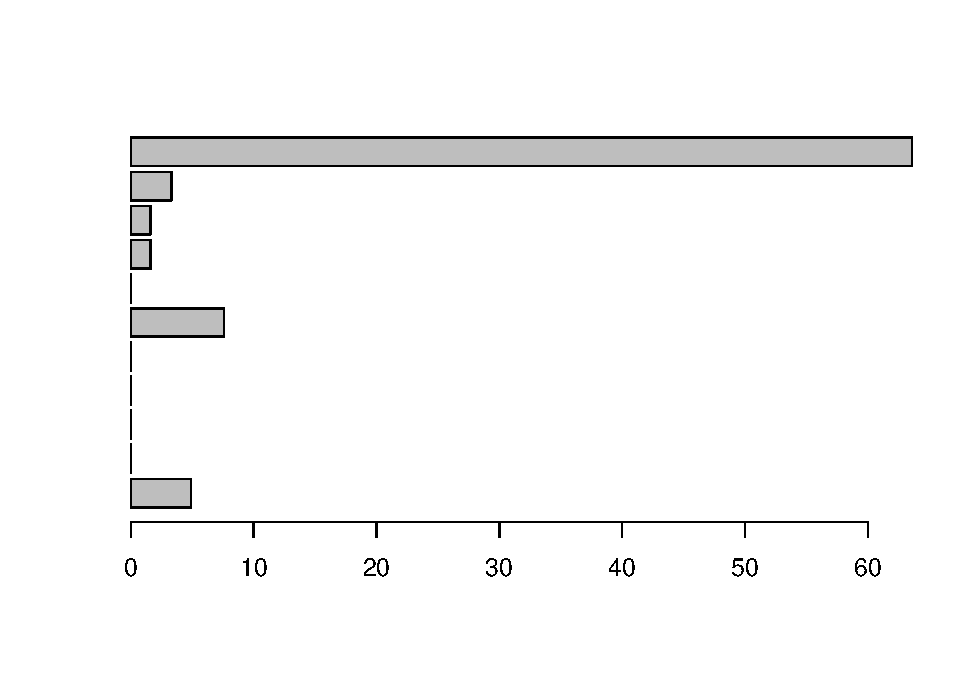
\includegraphics{diversificationInTheManagedFuturesUniverse_files/figure-latex/unnamed-chunk-30-1.pdf}

\begin{Shaded}
\begin{Highlighting}[]
\CommentTok{# create the table}
\NormalTok{knitr::}\KeywordTok{kable}\NormalTok{(}\KeywordTok{t}\NormalTok{(distributionAboveThreshold[systematicThreshold:}\DecValTok{100}\NormalTok{,}\DecValTok{1}\NormalTok{:}\DecValTok{2}\NormalTok{]))}
\end{Highlighting}
\end{Shaded}

\begin{longtable}[c]{@{}lrrrrrrrrrrr@{}}
\toprule
& 90 & 91 & 92 & 93 & 94 & 95 & 96 & 97 & 98 & 99 & 100\tabularnewline
\midrule
\endhead
\% systematic & 90.0 & 91 & 92 & 93 & 94 & 95.0 & 96 & 97.0 & 98.0 &
99.0 & 100.0\tabularnewline
\% of CTAs & 4.9 & 0 & 0 & 0 & 0 & 7.6 & 0 & 1.6 & 1.6 & 3.3 &
63.6\tabularnewline
\bottomrule
\end{longtable}

As can be seen in the above table, the vast majority of firms that
report a systematic component to their strategies claim that their
programs are 90\%, 95\%, or 100\% systematic. In the modeling section of
the paper we will model the relationships between

Each managed futures program uses a different level of leverage. The
level of allowed leverage is often a constraint set by investors. The
inverse of the collected quantity, `margin-to-equity', is the program
leverage. We extract the `margin-to-equity' as follows:

\begin{Shaded}
\begin{Highlighting}[]
\CommentTok{# extract the margin to equity data}
\NormalTok{query<-}\KeywordTok{paste0}\NormalTok{(}\StringTok{"SELECT * FROM altegris.cta_program_info "}\NormalTok{,}
  \StringTok{"WHERE column_type = 'investmentTermsAndInfo' AND "}\NormalTok{,}
  \StringTok{"column_name='Margin  Equity Ratio' "}\NormalTok{,}
  \StringTok{"ORDER BY cta_name,program_name,column_type;"}\NormalTok{)}
\CommentTok{# fetch the margin to equity}
\NormalTok{ctaMarginToEquity<-}\KeywordTok{dbGetQuery}\NormalTok{(dbHandle,query)}
\end{Highlighting}
\end{Shaded}

We convert the `margin-to-equity' to leverage as follows:

\begin{Shaded}
\begin{Highlighting}[]
\CommentTok{# convert the margin-to-equity to numeric}
\NormalTok{marginToEquity<-(}\KeywordTok{as.numeric}\NormalTok{(ctaMarginToEquity[,}\DecValTok{3}\NormalTok{]))}
\CommentTok{# convert the 'margin-to-equity' to leverage}
\NormalTok{leverage<-}\KeywordTok{round}\NormalTok{(}\DecValTok{1}\NormalTok{/(marginToEquity/}\DecValTok{100}\NormalTok{),}\DecValTok{1}\NormalTok{)}
\CommentTok{# find the min leverage}
\NormalTok{minLeverage<-}\KeywordTok{min}\NormalTok{(leverage,}\DataTypeTok{na.rm=}\OtherTok{TRUE}\NormalTok{)}
\CommentTok{# find the max leverage}
\NormalTok{maxLeverage<-}\KeywordTok{max}\NormalTok{(leverage,}\DataTypeTok{na.rm=}\OtherTok{TRUE}\NormalTok{)}
\CommentTok{# create the }
\NormalTok{xLeverage<-}\KeywordTok{seq}\NormalTok{(}\DataTypeTok{from=}\DecValTok{1}\NormalTok{,}\DataTypeTok{to=}\NormalTok{maxLeverage,}\DataTypeTok{by=}\DecValTok{1}\NormalTok{)}
\CommentTok{# find the frequency of different leverages}
\NormalTok{leverageFrequency<-}\KeywordTok{tabulate}\NormalTok{(leverage)}
\CommentTok{# great the graph}
\KeywordTok{barplot}\NormalTok{(leverageFrequency)}
\end{Highlighting}
\end{Shaded}

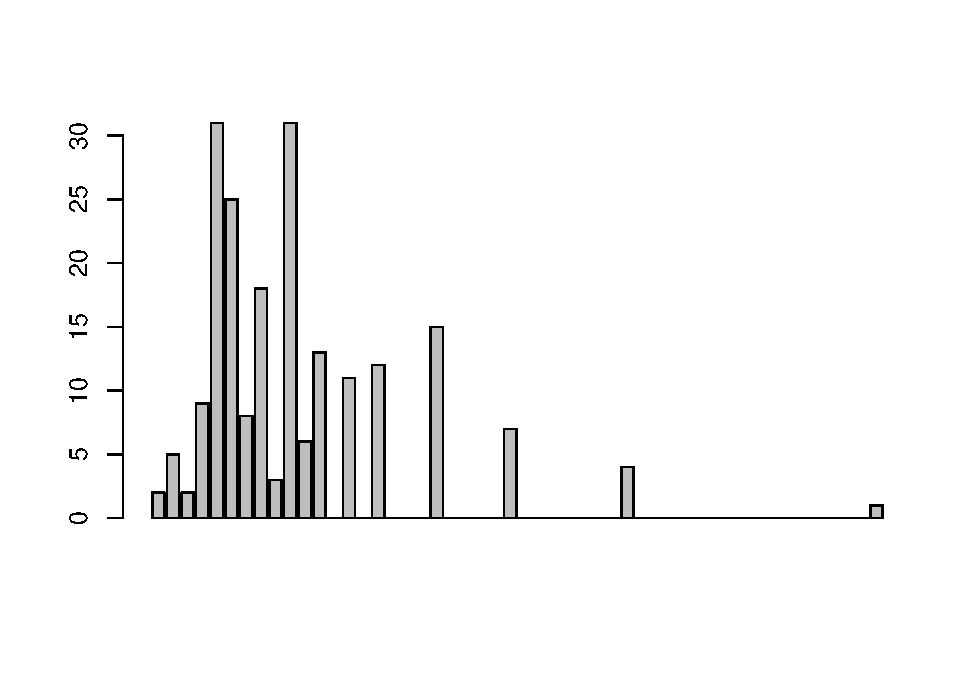
\includegraphics{diversificationInTheManagedFuturesUniverse_files/figure-latex/unnamed-chunk-32-1.pdf}

Finally, we extract the returns for a single managed futures program as
and create a summary of the performance as follows:

\begin{Shaded}
\begin{Highlighting}[]
\NormalTok{fetchMonthlyReturnsForCtaByProgramId <-}\StringTok{ }\NormalTok{function (dbHandle,programId)\{}
  \NormalTok{query<-}\KeywordTok{paste0}\NormalTok{(}\StringTok{"SELECT eom_date,monthly_return FROM cta_monthly_returns WHERE program_id="}\NormalTok{,}
    \NormalTok{programId)}
  \NormalTok{ctaReturns<-}\KeywordTok{dbGetQuery}\NormalTok{(dbHandle,query)}
  \NormalTok{eomDate<-}\KeywordTok{as.POSIXct}\NormalTok{(ctaReturns[,}\DecValTok{1}\NormalTok{])}
  \NormalTok{monthlyReturn<-ctaReturns[,}\DecValTok{2}\NormalTok{]/}\DecValTok{100}
  \NormalTok{ctaReturn<-}\KeywordTok{data.frame}\NormalTok{(eomDate,monthlyReturn,}\DataTypeTok{stringsAsFactors=}\OtherTok{FALSE}\NormalTok{)}
  \NormalTok{ctaReturn}
  \NormalTok{\}}
\end{Highlighting}
\end{Shaded}

\begin{Shaded}
\begin{Highlighting}[]
\NormalTok{minDate<-}\StringTok{"2005-01-01"}
\NormalTok{query<-}\KeywordTok{paste0}\NormalTok{(}\StringTok{"SELECT DISTINCT cta_name,program_name,program_id,MIN(eom_date) AS minDate "}\NormalTok{,}
  \StringTok{"FROM altegris.cta_monthly_returns WHERE eom_date<'"}\NormalTok{,}
  \NormalTok{minDate,}\StringTok{"' GROUP BY program_id ORDER BY cta_name;"}\NormalTok{)}
\NormalTok{ctaList<-}\KeywordTok{dbGetQuery}\NormalTok{(dbHandle,query)}
\NormalTok{programIds<-ctaList[}\StringTok{'program_id'}\NormalTok{]}
\NormalTok{ctaNames<-ctaList[}\StringTok{'cta_name'}\NormalTok{]}
\NormalTok{ctaPrograms<-ctaList[}\StringTok{'program_name'}\NormalTok{]}
\CommentTok{# remove some of the detail from the program name to make names shorter}
\NormalTok{ctaPrograms[,}\DecValTok{1}\NormalTok{]<-}\KeywordTok{gsub}\NormalTok{(}\StringTok{'*QEP*'}\NormalTok{,}\StringTok{''}\NormalTok{,ctaPrograms[,}\DecValTok{1}\NormalTok{])}
\NormalTok{ctaPrograms[,}\DecValTok{1}\NormalTok{]<-}\KeywordTok{gsub}\NormalTok{(}\StringTok{'*FRN*'}\NormalTok{,}\StringTok{''}\NormalTok{,ctaPrograms[,}\DecValTok{1}\NormalTok{])}
\NormalTok{ctaPrograms[,}\DecValTok{1}\NormalTok{]<-}\KeywordTok{gsub}\NormalTok{(}\StringTok{'}\CharTok{\textbackslash{}\textbackslash{}}\StringTok{**'}\NormalTok{,}\StringTok{''}\NormalTok{,ctaPrograms[,}\DecValTok{1}\NormalTok{])}
\NormalTok{ctaPrograms[,}\DecValTok{1}\NormalTok{]<-}\KeywordTok{gsub}\NormalTok{(}\StringTok{'*PROP*'}\NormalTok{,}\StringTok{''}\NormalTok{,ctaPrograms[,}\DecValTok{1}\NormalTok{])}
\NormalTok{ctaPrograms[,}\DecValTok{1}\NormalTok{]<-}\KeywordTok{gsub}\NormalTok{(}\StringTok{'*Program*'}\NormalTok{,}\StringTok{''}\NormalTok{,ctaPrograms[,}\DecValTok{1}\NormalTok{])}
\end{Highlighting}
\end{Shaded}

We can iterate over each program with historical data available prior to
2005-01-01 and extract the return data, adding each CTA program return
stream to the group.

\begin{Shaded}
\begin{Highlighting}[]
\CommentTok{# create the xts object to hold the group data}
\NormalTok{groupData <-}\StringTok{ }\KeywordTok{xts}\NormalTok{()}

\NormalTok{for (programIndex in }\DecValTok{1}\NormalTok{:}\KeywordTok{dim}\NormalTok{(programIds)[}\DecValTok{1}\NormalTok{])\{}
  \CommentTok{# get the program ID}
  \NormalTok{programId<-programIds[programIndex,}\DecValTok{1}\NormalTok{]}
  \CommentTok{# get the CTA name}
  \NormalTok{ctaName<-ctaList[programIndex,}\DecValTok{2}\NormalTok{]}
  \CommentTok{# fetch the program returns}
  \NormalTok{ctaReturn<-}\KeywordTok{fetchMonthlyReturnsForCtaByProgramId}\NormalTok{(dbHandle,programId)}
  \NormalTok{dataObject<-}\KeywordTok{xts}\NormalTok{(ctaReturn[,}\DecValTok{2}\NormalTok{],}\DataTypeTok{order.by=}\KeywordTok{as.POSIXct}\NormalTok{(ctaReturn[,}\DecValTok{1}\NormalTok{],}\DataTypeTok{format=}\StringTok{'%Y-%m-%d'}\NormalTok{))}
  \NormalTok{recentData<-}\KeywordTok{last}\NormalTok{(dataObject,}\StringTok{'10 year'}\NormalTok{)}
  \NormalTok{df<-}\KeywordTok{data.frame}\NormalTok{(}\DataTypeTok{date=}\KeywordTok{index}\NormalTok{(recentData),}\KeywordTok{coredata}\NormalTok{(recentData))}
  \CommentTok{# create the individual graph}
  \NormalTok{p1 <-}\StringTok{ }\KeywordTok{ggplot}\NormalTok{(ctaReturn, }\KeywordTok{aes}\NormalTok{(}\DataTypeTok{x=}\NormalTok{eomDate, }\DataTypeTok{y=}\KeywordTok{cumprod}\NormalTok{(}\DecValTok{1}\NormalTok{+monthlyReturn))) +}\StringTok{ }\KeywordTok{geom_line}\NormalTok{() +}\StringTok{ }
\StringTok{    }\KeywordTok{ggtitle}\NormalTok{(ctaName)+}\KeywordTok{xlab}\NormalTok{(}\StringTok{'Time'}\NormalTok{)+}\KeywordTok{ylab}\NormalTok{(}\StringTok{'Terminal Wealth Relative (TWR)'}\NormalTok{)+}\KeywordTok{theme_economist}\NormalTok{()+}
\StringTok{    }\KeywordTok{scale_colour_economist}\NormalTok{()}
  \CommentTok{# label the return data with the program ID}
  \KeywordTok{colnames}\NormalTok{(recentData)<-programId}
  \CommentTok{# add the individual progrma data to the group}
  \NormalTok{groupData <-}\StringTok{ }\KeywordTok{merge}\NormalTok{(groupData, recentData)}
\NormalTok{\}}
\NormalTok{groupDataDimension<-}\KeywordTok{dim}\NormalTok{(groupData)}
\end{Highlighting}
\end{Shaded}

We extract 112 months of CTA program return data for 76 distinct managed
futures programs.

Our data includes most of the managers with the most impressive track
records.

\begin{longtable}[c]{@{}llll@{}}
\toprule
& cta\_name & program\_name & minDate\tabularnewline
\midrule
\endhead
8 & Campbell \& Company, LP & Campbell Managed Futures &
1983-04-30\tabularnewline
1 & Abraham Trading Company & Abraham Diversified Program &
1990-01-31\tabularnewline
9 & Chesapeake Capital Corporation & Diversified Program \emph{QEP} &
1990-01-31\tabularnewline
22 & DUNN Capital Management, Inc. & World Monetary and Agriculture
(WMA) Program \emph{QEP} & 1990-01-31\tabularnewline
26 & EMC Capital Advisors LLC & Classic Program \emph{QEP} &
1990-01-31\tabularnewline
34 & Hawksbill Capital Management & Global Diversified Program
\emph{QEP} & 1990-01-31\tabularnewline
43 & Mark J. Walsh \& Company & Standard Program &
1990-01-31\tabularnewline
44 & Michael J. Frischmeyer, CTA & Michael J. Frischmeyer, CTA
\emph{CLSD} & 1990-01-31\tabularnewline
45 & Millburn Corporation & Diversified Program &
1990-01-31\tabularnewline
57 & Rabar Market Research, Inc. & Diversified Program \emph{QEP} &
1990-01-31\tabularnewline
\bottomrule
\end{longtable}

\subsection{Data Cleaning}\label{data-cleaning}

Data cleaning of the majority of the collected data pertaining to
manager and program information was beyond the scope of this project,
and as a result very little of this data was used in the modeling sector
of the paper.

The manager and program information collected is somewhat unstructured
and visual inspection of the managed futures website reveals many
reporting inconsistencies across managers. Our quick exploratory
analysis confirms that data is reported somewhat inconsistently by CTAs.
In particular, there appears to be very little validation of the manager
and program information submitted by CTAs. As a result, this part of the
collected data set requires a lot of cleaning and standardization before
it can be used effectively in our modeling.

In this section we provide a brief example of the types of
inconsistencies in the available progam and manager data.

We extract the information about the geographical region of each manager
as follows:

\begin{Shaded}
\begin{Highlighting}[]
\CommentTok{# create the query}
\NormalTok{query<-}\KeywordTok{paste0}\NormalTok{(}\StringTok{"SELECT DISTINCT column_value,COUNT(column_value) "}\NormalTok{,}
  \StringTok{"FROM altegris.cta_program_info WHERE column_type = 'address' "}\NormalTok{,}
  \StringTok{"AND column_name='Country' GROUP BY column_value  ORDER BY "}\NormalTok{,}
\StringTok{"column_value;"}\NormalTok{)}
\CommentTok{# extract the data}
\NormalTok{ctaCountry<-}\KeywordTok{dbGetQuery}\NormalTok{(dbHandle,query)}
\CommentTok{# create the table}
\KeywordTok{colnames}\NormalTok{(ctaCountry)<-}\KeywordTok{c}\NormalTok{(}\StringTok{'Country'}\NormalTok{,}\StringTok{'# of Programs'}\NormalTok{)}
\NormalTok{knitr::}\KeywordTok{kable}\NormalTok{(ctaCountry)}
\end{Highlighting}
\end{Shaded}

\begin{longtable}[c]{@{}lr@{}}
\toprule
Country & \# of Programs\tabularnewline
\midrule
\endhead
& 4\tabularnewline
Austria & 2\tabularnewline
Bahamas & 1\tabularnewline
Canada & 6\tabularnewline
Channel Islands & 1\tabularnewline
Cyprus & 1\tabularnewline
Finland & 4\tabularnewline
France & 2\tabularnewline
Germany & 1\tabularnewline
Hong Kong & 1\tabularnewline
Israel & 1\tabularnewline
Korea & 1\tabularnewline
Liechtenstein & 1\tabularnewline
Macedonia & 1\tabularnewline
Netherlands & 2\tabularnewline
Singapore & 1\tabularnewline
Spain & 2\tabularnewline
St.~Croix USVI & 1\tabularnewline
Switzerland & 6\tabularnewline
UK & 1\tabularnewline
United Kingdom & 16\tabularnewline
United Kingdon & 3\tabularnewline
United States & 35\tabularnewline
US & 1\tabularnewline
USA & 111\tabularnewline
\bottomrule
\end{longtable}

Spelling errors and single countries coded with multiple names (i.e.,
United Kingdom, United Kingdon, or UK for instance) are clear.

We can clean up the data as follows:

\begin{Shaded}
\begin{Highlighting}[]
\CommentTok{# replace empty with Unreported}
\NormalTok{ctaCountry[ctaCountry[,}\DecValTok{1}\NormalTok{]==}\StringTok{''}\NormalTok{,}\DecValTok{1}\NormalTok{]<-}\StringTok{'Unreported'}
\CommentTok{# reclassify US Virgin Islands as United States}
\NormalTok{ctaCountry[,}\DecValTok{1}\NormalTok{]<-}\KeywordTok{gsub}\NormalTok{(}\StringTok{'St. Croix USVI'}\NormalTok{,}\StringTok{'United States'}\NormalTok{,ctaCountry[,}\DecValTok{1}\NormalTok{])}
\CommentTok{# we clean up the US entries}
\NormalTok{ctaCountry[,}\DecValTok{1}\NormalTok{]<-}\KeywordTok{gsub}\NormalTok{(}\StringTok{'USA'}\NormalTok{,}\StringTok{'United States'}\NormalTok{,ctaCountry[,}\DecValTok{1}\NormalTok{])}
\NormalTok{ctaCountry[,}\DecValTok{1}\NormalTok{]<-}\KeywordTok{gsub}\NormalTok{(}\StringTok{'US'}\NormalTok{,}\StringTok{'United States'}\NormalTok{,ctaCountry[,}\DecValTok{1}\NormalTok{])}
\CommentTok{# we clean up the UK entries}
\NormalTok{ctaCountry[,}\DecValTok{1}\NormalTok{]<-}\KeywordTok{gsub}\NormalTok{(}\StringTok{'UK'}\NormalTok{,}\StringTok{'United Kingdom'}\NormalTok{,ctaCountry[,}\DecValTok{1}\NormalTok{])}
\NormalTok{ctaCountry[,}\DecValTok{1}\NormalTok{]<-}\KeywordTok{gsub}\NormalTok{(}\StringTok{'United Kingdon'}\NormalTok{,}\StringTok{'United Kingdom'}\NormalTok{,ctaCountry[,}\DecValTok{1}\NormalTok{])}
\CommentTok{# create the country factor}
\NormalTok{countryFactor <-}\StringTok{ }\KeywordTok{factor}\NormalTok{(ctaCountry[,}\DecValTok{1}\NormalTok{])}
\CommentTok{# redo the counts by country}
\NormalTok{cleanTable<-}\KeywordTok{aggregate}\NormalTok{(}\DataTypeTok{x=}\NormalTok{ctaCountry[,}\DecValTok{2}\NormalTok{],}\DataTypeTok{by=}\KeywordTok{list}\NormalTok{(countryFactor),}\DataTypeTok{FUN=}\StringTok{"sum"}\NormalTok{)}
\CommentTok{# compute the percent by region}
\NormalTok{countryPercent<-}\KeywordTok{round}\NormalTok{(cleanTable[,}\DecValTok{2}\NormalTok{]/}\KeywordTok{sum}\NormalTok{(cleanTable[,}\DecValTok{2}\NormalTok{]),}\DecValTok{4}\NormalTok{)}
\CommentTok{# add row names}
\KeywordTok{rownames}\NormalTok{(cleanTable)<-cleanTable[,}\DecValTok{1}\NormalTok{]}
\CommentTok{# create the table}
\NormalTok{cleanTable<-}\KeywordTok{cbind}\NormalTok{(cleanTable,countryPercent*}\DecValTok{100}\NormalTok{)}
\CommentTok{# remove country column}

\CommentTok{# label the columns}
\KeywordTok{colnames}\NormalTok{(cleanTable)<-}\KeywordTok{c}\NormalTok{(}\StringTok{'Country'}\NormalTok{,}\StringTok{'# of Programs'}\NormalTok{,}\StringTok{'% of Programs'}\NormalTok{)}
\CommentTok{# create the sort index}
\NormalTok{sortIndex<-}\KeywordTok{sort.int}\NormalTok{(cleanTable[,}\DecValTok{2}\NormalTok{],}\DataTypeTok{index.return=}\OtherTok{TRUE}\NormalTok{,}\DataTypeTok{decreasing=}\OtherTok{TRUE}\NormalTok{)}
\CommentTok{# write the clean table}
\NormalTok{knitr::}\KeywordTok{kable}\NormalTok{(cleanTable[sortIndex$ix,}\DecValTok{2}\NormalTok{:}\DecValTok{3}\NormalTok{])}
\end{Highlighting}
\end{Shaded}

\begin{longtable}[c]{@{}lrr@{}}
\toprule
& \# of Programs & \% of Programs\tabularnewline
\midrule
\endhead
United States & 148 & 71.84\tabularnewline
United Kingdom & 20 & 9.71\tabularnewline
Canada & 6 & 2.91\tabularnewline
Switzerland & 6 & 2.91\tabularnewline
Finland & 4 & 1.94\tabularnewline
Unreported & 4 & 1.94\tabularnewline
Austria & 2 & 0.97\tabularnewline
France & 2 & 0.97\tabularnewline
Netherlands & 2 & 0.97\tabularnewline
Spain & 2 & 0.97\tabularnewline
Bahamas & 1 & 0.49\tabularnewline
Channel Islands & 1 & 0.49\tabularnewline
Cyprus & 1 & 0.49\tabularnewline
Germany & 1 & 0.49\tabularnewline
Hong Kong & 1 & 0.49\tabularnewline
Israel & 1 & 0.49\tabularnewline
Korea & 1 & 0.49\tabularnewline
Liechtenstein & 1 & 0.49\tabularnewline
Macedonia & 1 & 0.49\tabularnewline
Singapore & 1 & 0.49\tabularnewline
\bottomrule
\end{longtable}

Now we can see that 71.84\% of the reporting managed futures programs
are operated out of the united states and 9.71\% are operated out of the
United Kingdom. The vast majority of programs are operated out of these
two regions (81.55\%). It is also notable that 1.94\% of managers do not
provide information about their geographical location.

\begin{Shaded}
\begin{Highlighting}[]
\CommentTok{# disconnect from the 'altegris' database}
\KeywordTok{dbDisconnect}\NormalTok{(dbHandle)}
\end{Highlighting}
\end{Shaded}

\begin{verbatim}
## [1] TRUE
\end{verbatim}

\pagebreak

\section{Modeling}\label{modeling}

In this section we provide a brief overview of the theory underlying our
application.

\subsection{Theory}\label{theory}

In the previous section, we provided an overview of the process used to
obtain the monthly returns for all distinct CTA programs available in
the Altegris managed futures database.

In this section, we provide a brief overview the theoretical
underpinnings of the modeling approach employed in our application. In
particular, we provide an outline of the eigen-decomposition underlying
the statistical factor analysis and outline an approach for determining
how many investment components contribute to each statistical factor.

\paragraph{Standardized Returns}\label{standardized-returns}

Standardization rescales a variable while preserving its order.

We denote the monthly return of the \(i^{th}\) investment for the
\(m^{th}\) month as \(r_{i,m}\) and define the standardized return as:

\[\hat{r}_{i,m}=\frac{\left( r_{i,m}-\bar{r}_{i,M}\right)}{\sigma(r_{i,M})}\]

Where

\(\hat{r}_{i,m}\) is the standardized return of the \(i^{th}\)
investment for the \(m^{th}\) month using data over the time interval
\(M\)

\(r_{i,m}\) is the observed return of the \(i^{th}\) investment for the
\(m^{th}\) month

\(\bar{r}_{i,M}=\frac{1}{M}\sum_{m=1}^{M}\left(\hat{r}_{m}\right)\) is
the mean of the return stream of the \(i^{th}\) investment over the time
interval \(M\)

\(\sigma(r_{i,M})=\) is the standard deviation of the returns for the
\(i^{th}\) investment over the time interval \(M\)

\paragraph{Correlations}\label{correlations}

We represent the standardized returns as an \(I\) x \(M\) matrix
\(\hat{R}\) with an empirical correlation matrix \(C\) defined as:

\[C = \frac{1}{M}\hat{R}\hat{R}^{T}\]

Where

\(T\) denotes the matrix transform

The correlation matrix (\(C\)) of returns (\(\hat{R}\)) and the
covariance matrix (\(\Sigma_{\hat{R}}\)) of standardized returns
(\(\hat{R}\)) are identical.

\subsubsection{Principal Component Analysis
(PCA)}\label{principal-component-analysis-pca}

The objective of principal component analysis (PCA) is to find a linear
transformation \(\Omega\) that maps a set of observed variables
\(\hat{R}\) into a set of uncorrelated variables \(F\). We define the
\(I\) x \(M\) statistical factor matrix as

\[F = \Omega\hat{R}\] {[}{]}

Where each row \(f_{k}\) (\(k = 1, \dots ,N\)) corresponds to a factor
\(F\) of \(\hat{R}\) and the transformation matrix \(\Omega\) has
elements \(\omega_{k,i}\). The first row of \(\omega_{1}\) (which
contains the first set of factor coefficients or `loadings') is chosen
such that the first factor (\(f_{1}\)) is aligned with the direction of
maximal variance in the \(I\)-dimensional space defined by \(\hat{R}\).
Each subsequent factor (\(f_{k}\)) accounts for as much of the remaining
variance of the standardized returns \(\hat{R}\) as possible, subject to
the constraint that the \(\omega_{k}\) are mutually orthogonal. The
vectors \(\omega_{k}\) are further constrained by requiring that
\(\omega_{k}\omega_{k}^{T}=1\) for all \(k\).

The correlation matrix \(C\) is an \(I\) x \(I\) diagonalizable
symmetric matrix that can be written in the form

\[C = \frac{1}{M}EDE^{T}\] {[}{]}

Where \(D\) is a diagonal matrix of eigenvalues \(d\) and \(E\) is an
orthogonal matrix of the corresponding eigenvectors.

The eigenvectors of the correlation matrix \(C\) correspond to the
directions of maximal variance such that \(\Omega=E^{T}\), and one finds
the statistical factors / principal components \(F\) using the
diagonalization in {[}{]}.

If the sign of every coefficient in a statistical factor \(f_{k}\) is
reversed, neither the variance of \(f_{k}\) nor the orthogonality of
\(\omega\) with respect to each of the other eigenvectors changes. For
this reason, the signs of factors (PCs) are arbitrary. This feature of
PCA can be problematic when we are interested in the temporal evolution
of factors.

\paragraph{Proportion of Variance}\label{proportion-of-variance}

The covariance matrix \(\Sigma_{F}\) for the statistical factor matrix
\(F\) can be written as:

\[\Sigma_{F}=\frac{1}{M}FF^{T}=\frac{1}{M}\Omega\hat{R}\hat{R}^{T} \Omega^{T} = D\]

Where \(D\) is the diagonal matrix of eigenvalues \(d\).

The total variance of the standardized returns \(\hat{R}\) for the \(I\)
investments is then

\[\sum_{i=1}^{I}\sigma^{2}(\hat{r}_{i})=tr(\Sigma_{\hat{R}})=\sum_{i=1}^{I}d_{i}=\sum_{i=1}^{N}\sigma^{2}(f_{i})=tr(D)=I\]

Where \(\Sigma_{\hat{R}}\) is the covariance matrix for \(\hat{R}\)

\(\sigma^{2}(\hat{r_{i}})=1\) is the variance of the vector
\(\hat{r_{i}}\) of standardized returns for investment \(i\).

The proportion of the total variance in \(\hat{R}\) explained by the
\(k^{th}\) factor is then

\[\frac{\sigma^{2}(f_{k})}{\Sigma_{i=1}^{I}\sigma^{2}(\hat{r_{i}})}=\frac{d_{k}}{\Sigma_{i=1}^{I}d_{k}}=\frac{d_{k}}{I}\]

The proportion of the variance from the \(k^{th}\) factor is equal to
the ratio of the \(k^{th}\) largest eigenvalue \(d_{k}\) to the number
of investments \(I\).

\paragraph{Number of Significant
Components}\label{number-of-significant-components}

To determine how many statistical factors are needed to describe the
correlations between investments, many methods have been proposed. There
is no widespread agreement on an optimal approach. In this paper we
focus on the first factor where we are able to find a clear economic
interpretation of the factor.

\paragraph{Significant Statistical Factor
Coefficients}\label{significant-statistical-factor-coefficients}

An increase in the variance associated with a factor can be the result
of increases in the correlations among only a few investment programs
(which then have large factor coefficients) or an effect in which many
investment programs begin to make significant contributions to the
factor, This is an important distinction, because the two types of
changes have very different implications for portfolio management. It
becomes much more difficult to reduce risk by diversifying across
different investment when correlations between all investments increase.
In contrast, increases in correlations within an investment type that
are not accompanied by increases in correlations between investment
types have a less significant impact on diversification.

\subparagraph{Inverse Participation Ratio
(IPR)}\label{inverse-participation-ratio-ipr}

The inverse participation ratio \(I_{k}\) of the \(k^{th}\) factor
\(\omega_{k}\) is defined as:

\[IPR_{k}=\sum_{i=1}^{I}\left( \omega_{k,i}\right)^{4}\]

The IPR quantifies the reciprocal of the number of elements that make a
significant contribution to each eigenvector.

The behavior of the IPR is bounded by two cases:

{[}1{]} An eigenvector with identical contributions
\(\omega_{k,i}=frac{1}{\sqrt{I}}\) from all \(I\) investments has
\(IPR_{k}=\frac{1}{I}\)

{[}2{]} An eigenvector with a single factor \(\omega_{k,i}=1\) and
remaining factors equal to zero has \(IPR=1\)

The inverse of the IPR - the so-called participation ratio - provides a
more intuitive measure of the significance of a given factor as a large
\(PR\) indicates that many investments contribute to the factor, while a
small \(PR\) signals that few investments contribute to the factor:

\(PR = \frac{1}{IPR_{k}}\)

The participation ratio quantifies the number of eigenvector components
that participate in a factor and provides a measure of concentration.

The bigger a PA is, more the participants the statistical factor has,
the more uniformly distributed the participation is and the more
correlations are driven by the statistical facotr.

Participation ratios facilitate the identification of statistical
facotrs that represent macroeconomic scenarios, namely thos with with
many participants. They also help us identify factors that represent
microeconomic scenarios, namely factors with few participants.

\subsubsection{Portfolio Factor Sensitivities and Coherent Scenario
Analysis}\label{portfolio-factor-sensitivities-and-coherent-scenario-analysis}

We can use our factor model to determine the impact of an increase in
the proportion of variance described by any given statistical factor on
our correlation matrix. By perturbing the eigenvalues up and down and
applying the appropriate re-normalizations we create data-coherent
approach to generating changes in the correlations driven by a common
factor.

The following three functions are used to implement the sensitivity
analysis in the application section of the paper.

\begin{Shaded}
\begin{Highlighting}[]
\NormalTok{perturbCorrelation<-function (shockFactor,factorIndex,eigenvalues,eigenvectors)\{}
  \CommentTok{# create the hash to store the results}
  \NormalTok{scenario<-}\KeywordTok{hash}\NormalTok{()}
  \NormalTok{scenarioEigenvalues <-}\StringTok{ }\NormalTok{eigenvalues}
  \NormalTok{scenarioEigenvalues[factorIndex] <-}\StringTok{ }\NormalTok{eigenvalues[factorIndex] *}\StringTok{ }\NormalTok{shockFactor}
  \NormalTok{C1 <-}\StringTok{ }\NormalTok{eigenvectors %*%}\StringTok{ }\KeywordTok{diag}\NormalTok{(scenarioEigenvalues) %*%}\StringTok{ }\KeywordTok{t}\NormalTok{(eigenvectors)}
  \CommentTok{# extract the variance}
  \NormalTok{V <-}\StringTok{ }\KeywordTok{diag}\NormalTok{(}\DecValTok{1}\NormalTok{/}\KeywordTok{sqrt}\NormalTok{(C1))}
  \CommentTok{# normalize the correlation matrix}
  \NormalTok{C2 <-}\StringTok{ }\KeywordTok{diag}\NormalTok{(V) %*%}\StringTok{ }\NormalTok{C1 %*%}\StringTok{ }\KeywordTok{diag}\NormalTok{(V)}
  \CommentTok{# eigen decomposition}
  \NormalTok{scenarioDecomposition=}\KeywordTok{eigen}\NormalTok{(C2)}
  \CommentTok{# extract the stressed eigenvalues}
  \NormalTok{eigenvaluesF=scenarioDecomposition$values}
  \CommentTok{# extract the stressed eigenvector}
  \NormalTok{eigenvectorF=scenarioDecomposition$vectors}
  \CommentTok{# number of factors}
  \NormalTok{numberOfFactors<-}\KeywordTok{sum}\NormalTok{(eigenvaluesF)}
  \CommentTok{# compute the proportion of variance}
  \NormalTok{scenarioProportionOfVariance<-eigenvaluesF/numberOfFactors}
  \CommentTok{# store the correlation matrix}
  \NormalTok{scenario[}\StringTok{'correlation'}\NormalTok{]<-C2}
  \CommentTok{# store the proportion of variance}
  \NormalTok{scenario[}\StringTok{'proportionOfVariance'}\NormalTok{]<-scenarioProportionOfVariance}
  \CommentTok{# return the scenario}
  \NormalTok{scenario}
\NormalTok{\}}
\end{Highlighting}
\end{Shaded}

\begin{Shaded}
\begin{Highlighting}[]
\NormalTok{perturbFactorCorrelation <-}\StringTok{ }\NormalTok{function (factorIndex,eigenvalues,eigenvectors)\{}
  \CommentTok{# create the hash}
  \NormalTok{scenarios<-}\KeywordTok{hash}\NormalTok{()}
  \CommentTok{# create shock scenarios}
  \NormalTok{shockFactors<-}\KeywordTok{seq}\NormalTok{(}\DataTypeTok{from=}\FloatTok{0.2}\NormalTok{,}\DataTypeTok{to=}\DecValTok{5}\NormalTok{,}\DataTypeTok{by=}\FloatTok{0.2}\NormalTok{)}

  \CommentTok{# iterate over shock factors}
  \NormalTok{for (shockIndex in }\KeywordTok{seq_along}\NormalTok{(shockFactors))\{}
    \CommentTok{# extract the shock}
    \NormalTok{shockFactor<-shockFactors[shockIndex]}
    \CommentTok{# increase the importance of the factorIndex factor}
    \NormalTok{scenario<-}\KeywordTok{perturbCorrelation}\NormalTok{(shockFactor,factorIndex,eigenvalues,eigenvectors)}
    \CommentTok{# store the correlation}
    \NormalTok{scenarios[}\KeywordTok{paste0}\NormalTok{(}\StringTok{'scenario_'}\NormalTok{,shockIndex)]<-scenario}
  \NormalTok{\}}
  \CommentTok{# return scenarios}
  \NormalTok{scenarios}
\NormalTok{\}}
\end{Highlighting}
\end{Shaded}

\begin{Shaded}
\begin{Highlighting}[]
\NormalTok{factorBasedCorrelationSensitivity<-function (numberOfFactors,C)\{}
  \CommentTok{# find the number of rows and columns}
  \NormalTok{dimension<-}\KeywordTok{dim}\NormalTok{(C)}
  \CommentTok{# create the storage matrix}
  \NormalTok{sensitivity<-}\KeywordTok{matrix}\NormalTok{(}\DecValTok{0}\NormalTok{,numberOfFactors,dimension[}\DecValTok{2}\NormalTok{])}
  \CommentTok{# compute the eigendecomposition}
  \NormalTok{decomposition=}\KeywordTok{eigen}\NormalTok{(C)}
  \CommentTok{# extract eigenvalues}
  \NormalTok{eigenvalues=decomposition$values}
  \CommentTok{# extract eigenvectors}
  \NormalTok{eigenvectors=decomposition$vectors}
  \CommentTok{# find the proportion of variance}
  \NormalTok{proportionOfVariance=eigenvalues/}\KeywordTok{length}\NormalTok{(eigenvalues)}
  \CommentTok{# find the explained variance}
  \NormalTok{explainedVariance=}\KeywordTok{cumsum}\NormalTok{(proportionOfVariance)}
  \CommentTok{# create hash}
  \NormalTok{scenariosByFactor<-}\KeywordTok{hash}\NormalTok{()}
  
  \CommentTok{# iterate over each factor}
  \NormalTok{for (factorIndex in }\DecValTok{1}\NormalTok{:numberOfFactors)\{}
    \CommentTok{# perturb the factor}
    \NormalTok{scenarios<-}\KeywordTok{perturbFactorCorrelation}\NormalTok{(factorIndex,eigenvalues,eigenvectors)}
    \NormalTok{scenariosByFactor[}\KeywordTok{paste0}\NormalTok{(}\StringTok{'factor_'}\NormalTok{,factorIndex)]<-scenarios}
    \CommentTok{#}
    \NormalTok{scenarioIndices<-}\KeywordTok{sort}\NormalTok{(}\KeywordTok{as.numeric}\NormalTok{(}\KeywordTok{gsub}\NormalTok{(}\StringTok{'scenario_'}\NormalTok{,}\StringTok{''}\NormalTok{,}
      \KeywordTok{names}\NormalTok{(scenariosByFactor[}\KeywordTok{paste0}\NormalTok{(}\StringTok{'factor_'}\NormalTok{,factorIndex)]))))}
    \NormalTok{\}}
  \NormalTok{scenariosByFactor}
\NormalTok{\}}
\end{Highlighting}
\end{Shaded}

\subsection{Applicaton}\label{applicaton}

In this section we apply the theory outlined in the above section. In
particular, we build a simple factor model of managed futures program
returns and use it to create sensitivities that map the proportion of
total variance in the investment universe to portfolio variation. This
sensitivity allows us to monitor the time-varying proportion of variance
explained by the first few statistical factors and instantly convert
these measures of market state into portfolio variability. This is
particularly useful during times of crisis when the importance of the
first few factors increase significantly.

\subsubsection{Data Preprocessing}\label{data-preprocessing}

Prior to any modeling, we standardize the managed futures program
returns.

We compute the correlation

\subsubsection{Statistical Factor
Analysis}\label{statistical-factor-analysis}

We now decompose the correlation matrix into statistical factors.

The top 5 factors explain a very significant proportion of the total
variance.

\begin{longtable}[c]{@{}lrr@{}}
\toprule
Factors & Proportion of Variance & Cumulative Proportion of
Variance\tabularnewline
\midrule
\endhead
Factor 1 & 36.8 & 36.8\tabularnewline
Factor 2 & 8.8 & 45.7\tabularnewline
Factor 3 & 6.5 & 52.1\tabularnewline
Factor 4 & 4.0 & 56.1\tabularnewline
Factor 5 & 3.6 & 59.8\tabularnewline
Factor 6 & 3.0 & 62.8\tabularnewline
Factor 7 & 2.5 & 65.3\tabularnewline
Factor 8 & 2.2 & 67.6\tabularnewline
Factor 9 & 2.2 & 69.8\tabularnewline
Factor 10 & 2.0 & 71.8\tabularnewline
\bottomrule
\end{longtable}

The first statistical factor accounts for 37\% of the variation of the
sytems. Indeed the first factor is the most significant by far. The
second factor acounts for another 9\% of the variation, and the third
component accounts for 6\% more. Indeed, the first three factors
together account for 52\% of the variation. The first 10 factors acount
for 37\% proportion of the variation in the system. By focusing on just
three factors we can understand a very significant proportion of the
total variation in the managed futures universe under study.

When we sort the factor loadings by the first factor we can see that the
all but two (relative value) funds contribute to the first factor, with
the long- and medium- term trend-following funds making the strongest
contributions and the volatility selling, short-term and relative value
programs having small or negative loadings.

The ten smallest factor loadings are:

\begin{longtable}[c]{@{}lllr@{}}
\caption{Smallest Factor 1 Loadings}\tabularnewline
\toprule
& Manager Name & Program Name & Factor 1\tabularnewline
\midrule
\endfirsthead
\toprule
& Manager Name & Program Name & Factor 1\tabularnewline
\midrule
\endhead
18 & Doherty Advisors, LLC & Relative Value Volatility 2X &
-0.0434\tabularnewline
19 & Doherty Advisors, LLC & Relative Value Volatility 1X &
-0.0410\tabularnewline
74 & Warrington Asset Management Corp. & Strategic Fund &
-0.0228\tabularnewline
52 & Paskewitz Asset Management, LLC & Contrarian 3X Stock Index &
-0.0209\tabularnewline
50 & Omni Trading, LLC & S\&P 500 Option Overwriting &
-0.0039\tabularnewline
54 & Quantitative Investment Management, LLC & Global &
0.0023\tabularnewline
42 & Kinkopf Capital Management, LLC & Kinkopf S\&P &
0.0034\tabularnewline
68 & Systematic Alpha Management LLC & Systematic Alpha Futures &
0.0044\tabularnewline
2 & AgTech Trading Company & Ag Trading & 0.0052\tabularnewline
32 & Goldman Management, Inc. & Goldman Management Stock Index Futures &
0.0079\tabularnewline
\bottomrule
\end{longtable}

The ten largest factor loadings are:

\begin{longtable}[c]{@{}lllr@{}}
\caption{Largest Factor 1 Loadings}\tabularnewline
\toprule
& Manager Name & Program Name & Factor 1\tabularnewline
\midrule
\endfirsthead
\toprule
& Manager Name & Program Name & Factor 1\tabularnewline
\midrule
\endhead
75 & Welton Investment Partners LLC & Global Directional Portfolio &
0.1514\tabularnewline
41 & Kelly Angle Inc. & Genesis & 0.1516\tabularnewline
66 & SMN Investment Services GmbH & Diversified Futures &
0.1522\tabularnewline
28 & Estlander \& Partners Ltd. & Alpha Trend & 0.1522\tabularnewline
22 & DUNN Capital Management, Inc. & World Monetary and Agriculture
(WMA) & 0.1525\tabularnewline
1 & Abraham Trading Company & Abraham Diversified &
0.1530\tabularnewline
49 & Mulvaney Capital Management Ltd & Global Diversified &
0.1550\tabularnewline
38 & ISAM - International Standard Asset Management & Systematic &
0.1563\tabularnewline
56 & Quest Partners LLC & AlphaQuest Original (AQO) &
0.1586\tabularnewline
26 & EMC Capital Advisors LLC & Classic & 0.1603\tabularnewline
\bottomrule
\end{longtable}

The first factor can be thus thought of as a `long directional
volatility' factor.

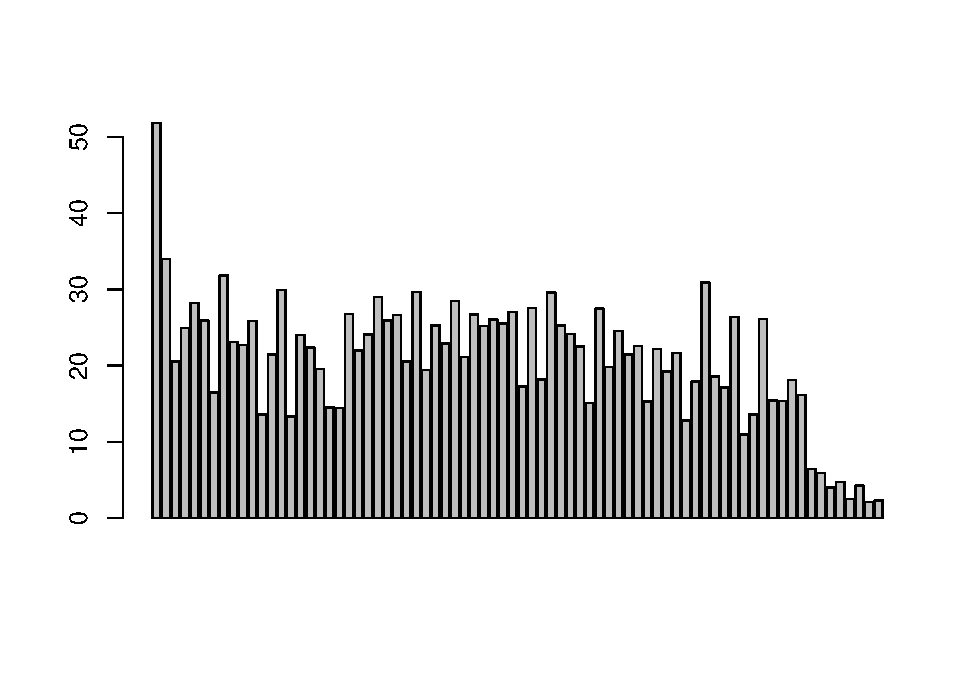
\includegraphics{diversificationInTheManagedFuturesUniverse_files/figure-latex/unnamed-chunk-53-1.pdf}

Using the participation ratio defined in the previous section, we see
that 52 components make significant contributions to the first factor.
This is in strong contrast to the other factors where the number of
components making significant contribtions is between 2 and 34.

Although more examination of the factors would be required to get an
deeper intuitive sense of the factors, we proceed to illustrating how
our simple statistical factor model can be used to create sensitivities
linking

\paragraph{Determining the Impact of Factors on Portfolio
Variability}\label{determining-the-impact-of-factors-on-portfolio-variability}

We can perturb the importance of the first factor up and down and use
our equation for portfolio standard deviation to determine the impact of
on a portfolio with equal allocations to our 76 managed futures
programs.

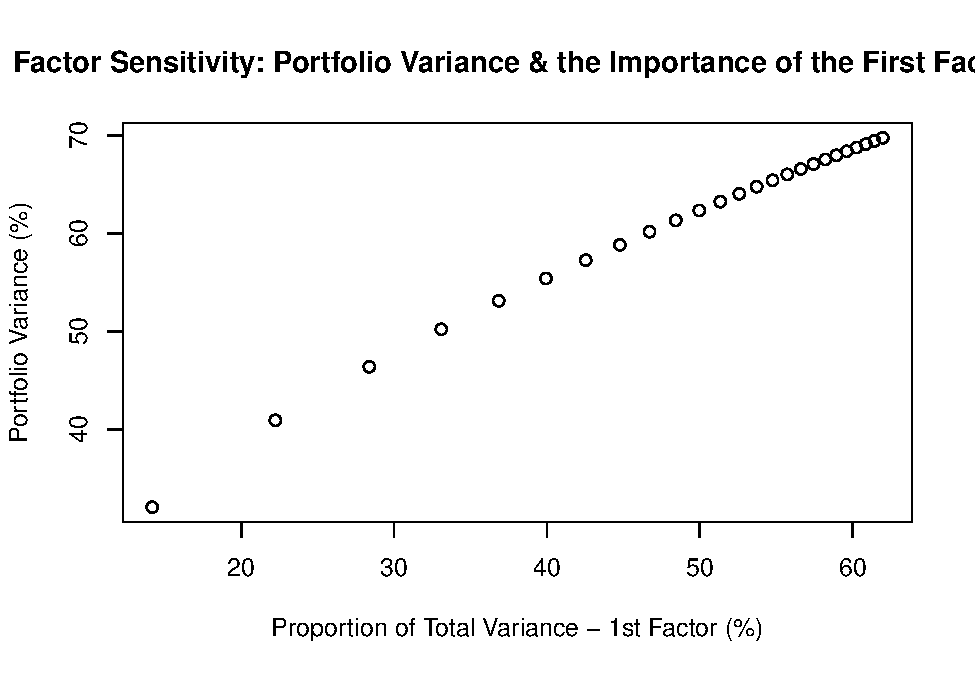
\includegraphics{diversificationInTheManagedFuturesUniverse_files/figure-latex/unnamed-chunk-54-1.pdf}

As the proportion of the portfolio variance explained by the first
factor increases, the portfolio variance increases. Using this
sensitivity measure, we can track the current proportion of variance
explained by the first factor and instantly know the impact on the
variation of portfolio returns.

\section{Conclusions}\label{conclusions}

Our factor analysis revealed a very significant proportion of the total
variance of the modeled managed futures universe can be captured by a
single statistical factor. This factor corresponds to a very intuitive
scenario. The sensitivity analysis developed - given the intuitive
interpretation of the first factor - can be used better understand
variation in the managed futures universe and can be used to identify
programs that behave differently.

\pagebreak

\section{References}\label{references}

{[}1{]} C. Bacon {[}2008{]}, Practical Portfolio Performance Measurement
and Attribution, \(2^{nd}\) Ed, John Wiley \& Sons, Inc.

{[}2{]} D. J. Fenn, N. F. Johnson, N. S. Jones, M. McDonald, M. A.
Porter, S. Williams {[}2011{]}, Temporal evolution of financial-market
correlations, Physical Review E 84, 026109

{[}3{]} F. J. Fabozzi, S. M. Focardi, P. N. Kolm {[}2010{]},
Quantitative Equity Investing: Techniques and Strategies (Frank J.
Fabozzi Series), John Wiley \& Sons, Inc.

{[}4{]} N. Fenton, M. Neil {[}2013{]}, Risk Assessment and Decision
Analysis With Bayesian Networks, CRC Press

{[}5{]} D. Koller, N. Friedman {[}2009{]}, Probabilistic graphical
models: principles and techniques, MIT press.

{[}6{]} A. Golub and Z. Guo {[}2012{]}, Correlation Stress Tests Under
the Random Matrix Theory: An Empirical Implementation to the Chinese
Market

{[}7{]} A Meucci {[}2009{]}, Risk and Asset Allocation, \(1^{st}\) Ed,
Springer Berlin Heidelberg

{[}8{]} R. Rebonato {[}2010{]}, Plight of the Fortune Tellers: Why We
Need to Manage Financial Risk Differently, Princeton University Press

{[}9{]} R. Rebonato {[}2010{]}, Coherent Stress Testing: A Bayesian
Approach to the Analysis of Financial Stress , John Wiley \& Sons, Inc.

{[}10{]} R. Rebonato and A. Denev {[}2014{]}, Portfolio Management Under
Stress: A Bayesian-net Approach to Coherent Asset Allocation, Cambridge
University Press

{[}11{]} D. Skillicorn {[}2007{]}, Understanding Complex Datasets: Data
Mining with Matrix Decompositions, Chapman and Hall/CRC

{[}12{]} R. Vince {[}2007{]}, The Handbook of Portfolio Mathematics:
Formulas for Optimal Allocation and Leverage, John Wiley \& Sons, Inc.

\pagebreak

\section{Appendix A: GitHub
Repository}\label{appendix-a-github-repository}

All of the R code used to produce this paper can be found in the
following github repository:

\url{https://github.com/dgn2/managed_futures}

The .Rmd is available to:

\begin{itemize}
\item
  extract CTA manager, program, and monthly return data from the
  Altegris managed futures website
\item
  create a MySQL database with tables to store extracted CTA manager,
  program, and monthly return data
\item
  load CTA manager, program, and monthly return data to the MySQL
  database
\item
  conduct limited exploratory analysis of the data
\item
  conduct limited cleaning of the data used in subsequent statistical
  modeling
\item
  estimate statistical factors based on the monthly returns of a select
  set of CTA programs
\item
  compute sensitivities
\end{itemize}

The github repository also includes the .Rmd file used to generate the
.pdf working paper file.

\pagebreak

\section{Appendix B: Data Dictionary}\label{appendix-b-data-dictionary}

The data dictionary for the data extracted from the Altegris managed
futures website can be found in the github repository:

\url{https://github.com/dgn2/managed_futures}

\pagebreak

\section{Apprendix C: Fundamental Laws of
Investing}\label{apprendix-c-fundamental-laws-of-investing}

\subsection{Importance of Capital
Preservation}\label{importance-of-capital-preservation}

The amount to recover from a loss increases geometrically with the
magnitude of the loss.

\[G = \left(\frac{1}{1-L}\right)-1\]

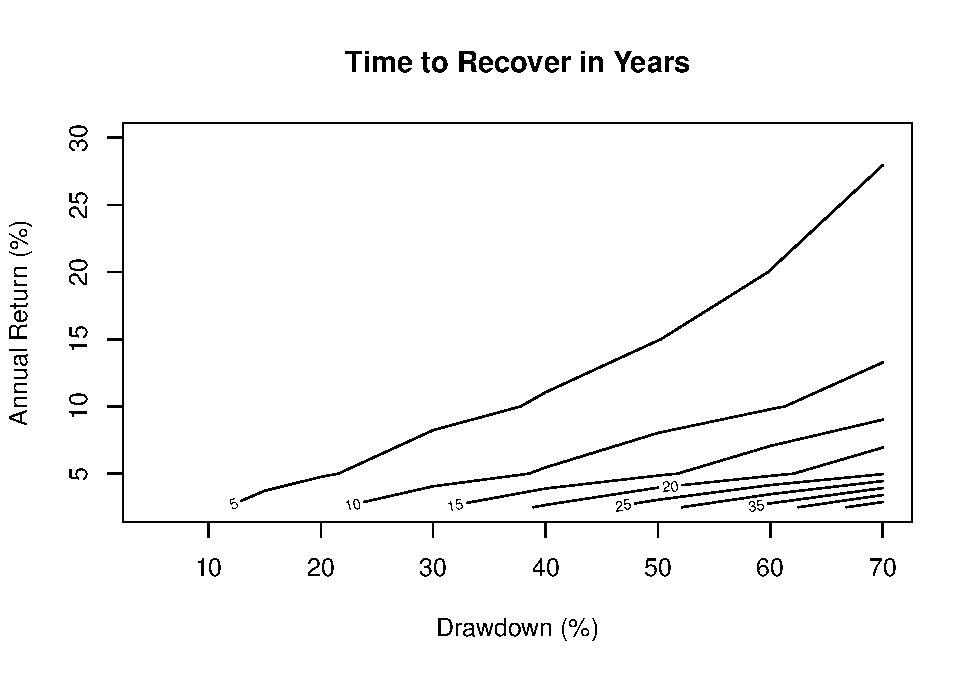
\includegraphics{diversificationInTheManagedFuturesUniverse_files/figure-latex/unnamed-chunk-55-1.pdf}

\begin{longtable}[c]{@{}lrrrrrr@{}}
\toprule
& 2.5 & 5 & 10 & 15 & 20 & 30\tabularnewline
\midrule
\endhead
5 & 2.08 & 1.05 & 0.54 & 0.37 & 0.28 & 0.20\tabularnewline
10 & 4.27 & 2.16 & 1.11 & 0.75 & 0.58 & 0.40\tabularnewline
15 & 6.58 & 3.33 & 1.71 & 1.16 & 0.89 & 0.62\tabularnewline
20 & 9.04 & 4.57 & 2.34 & 1.60 & 1.22 & 0.85\tabularnewline
30 & 14.44 & 7.31 & 3.74 & 2.55 & 1.96 & 1.36\tabularnewline
40 & 20.69 & 10.47 & 5.36 & 3.65 & 2.80 & 1.95\tabularnewline
50 & 28.07 & 14.21 & 7.27 & 4.96 & 3.80 & 2.64\tabularnewline
60 & 37.11 & 18.78 & 9.61 & 6.56 & 5.03 & 3.49\tabularnewline
70 & 48.76 & 24.68 & 12.63 & 8.61 & 6.60 & 4.59\tabularnewline
\bottomrule
\end{longtable}

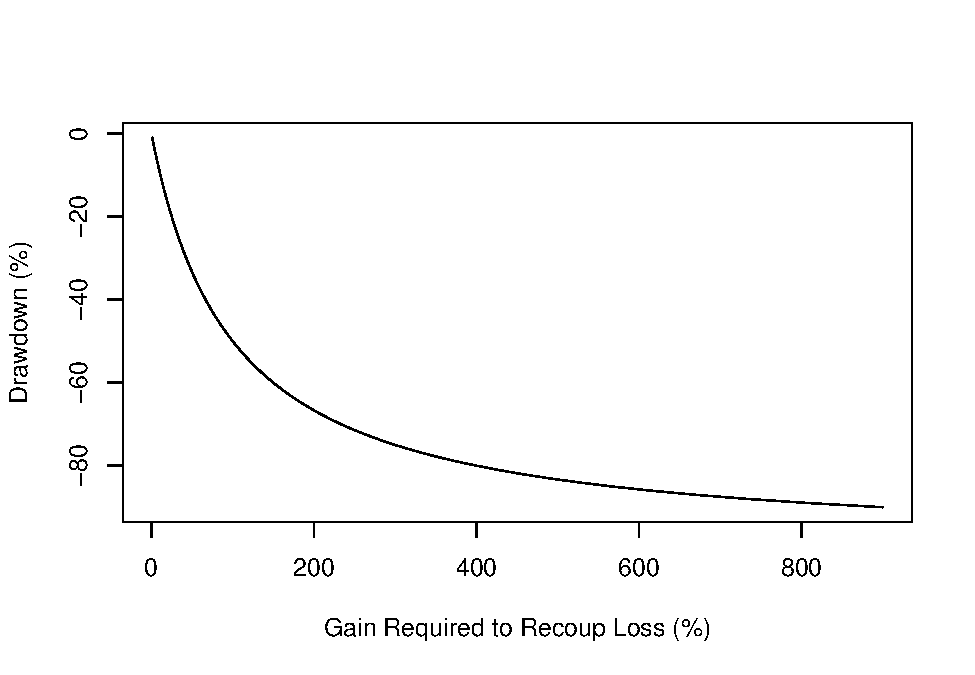
\includegraphics{diversificationInTheManagedFuturesUniverse_files/figure-latex/unnamed-chunk-56-1.pdf}

A loss of 20\% requires a gain of 25\% to recoup the loss.

A loss of 30\% requires a gain of 43\% to recoup the loss.

A loss of 40\% requires a gain of 67\% to recoup the loss.

A loss of 50\% requires a gain of 100\% to recoup the loss.

A loss of 60\% requires a gain of 150\% to recoup the loss.

A loss of 70\% requires a gain of 233\% to recoup the loss.

\end{document}
